% ----------------------------------------------------------
% Análise dos Resultados
% 
% ----------------------------------------------------------

\chapter[Desenvolvimento]{Desenvolvimento}

A pesquisa realizada proporcionou uma compreensão mais profunda dos potenciais clientes e usuários da solução, os quais são, no caso, jovens entre 19 e 22 anos. No contexto, os clientes e os usuários da solução são as mesmas pessoas, já que quem paga é também quem utiliza. Portanto, devido à inexistência de distinção entre usuários e clientes, a implementação do MVP é única.

\section{Requisitos do Sistema}
Como usuário do aplicativo FiMa, quero poder gerenciar minhas finanças de forma prática e transparente, tendo uma visão geral das despesas e receitas, podendo definir e acompanhar metas, recebendo sugestões de melhoria com base nos meus dados, para que eu atinja minhas metas e objetivos.

\subsection{Estória do Painel de Visão Geral}
Como usuário do aplicativo FiMa, quero ver um painel de visão geral das minhas finanças que exiba meu saldo atual, despesas, receitas e histórico, para ter melhor visibilidade.

\subsection{Estória de Definição de Metas}
Como usuário do aplicativo FiMa, quero poder definir metas financeiras, como economizar para uma viagem, um carro novo ou uma emergência, para que eu possa acompanhar meu progresso em relação a essas metas.

\subsection{Estória de Acompanhamento de Metas}
Como usuário do aplicativo FiMa, quero ser capaz de acompanhar meu progresso em relação às metas financeiras definidas, recebendo atualizações regulares sobre o quanto já alcancei e o que falta para atingir cada meta.

\subsection{Estória de Categorização de Despesas e Receitas}
Como usuário do aplicativo FiMa, quero poder categorizar minhas despesas e receitas, para que eu possa entender melhor para onde meu dinheiro está indo.

\subsection{Estória de Segurança e Privacidade}
Como usuário do aplicativo FiMa, quero ter a garantia de que meus dados financeiros serão protegidos adequadamente e que a privacidade das minhas informações será respeitada em conformidade com a Lei Geral de Proteção de Dados.

\section{Cronograma de Projeto}

Diagrama de Gantt contendo as atividades, papéis e responsabilidades dos participantes do grupo, conforme descrito na figura 11.

    \vspace{\baselineskip}
    \begin{center}
        \begin{minipage}{\textwidth}
            %\centering
            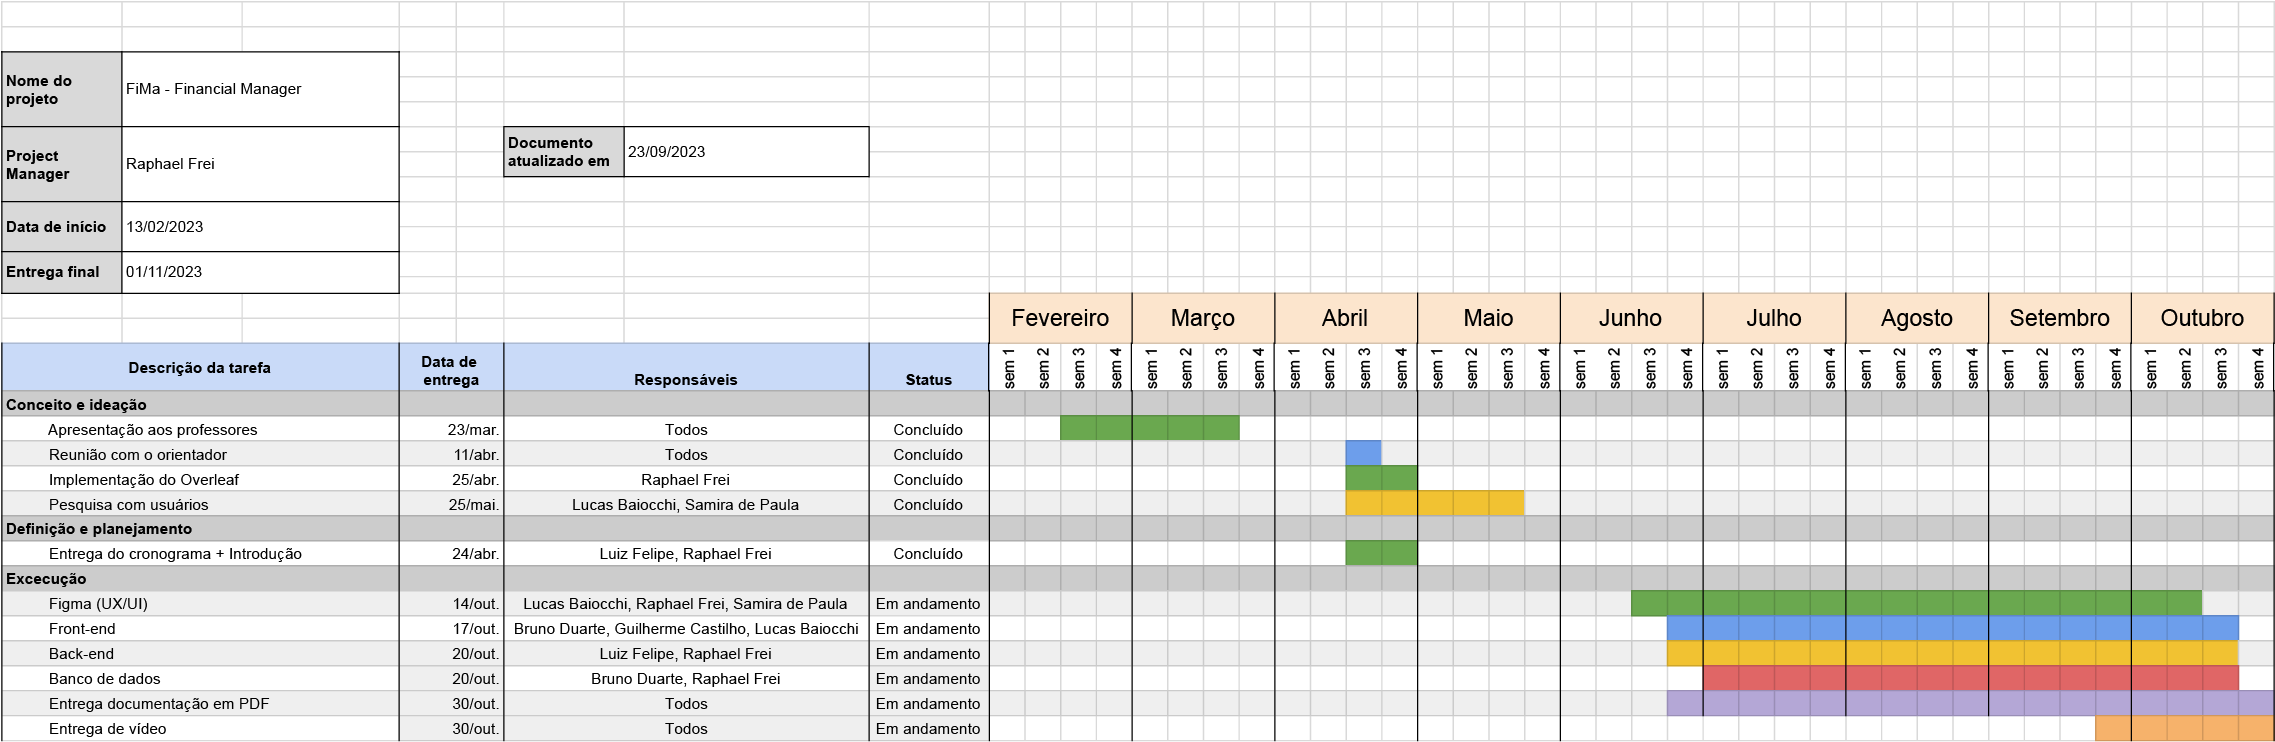
\includegraphics[scale=0.35]{figs/gantt.png}
            \captionof{figure}{Gráfico de Gantt}
            \label{fig:gantt}
        \end{minipage}
    \end{center}
    

\section{Desenho da Arquitetura do Software}

A figura 12 abaixo contém a arquitetura geral do sistema.

    \vspace{\baselineskip}
    \begin{center}
        \begin{minipage}{\textwidth}
            \centering
            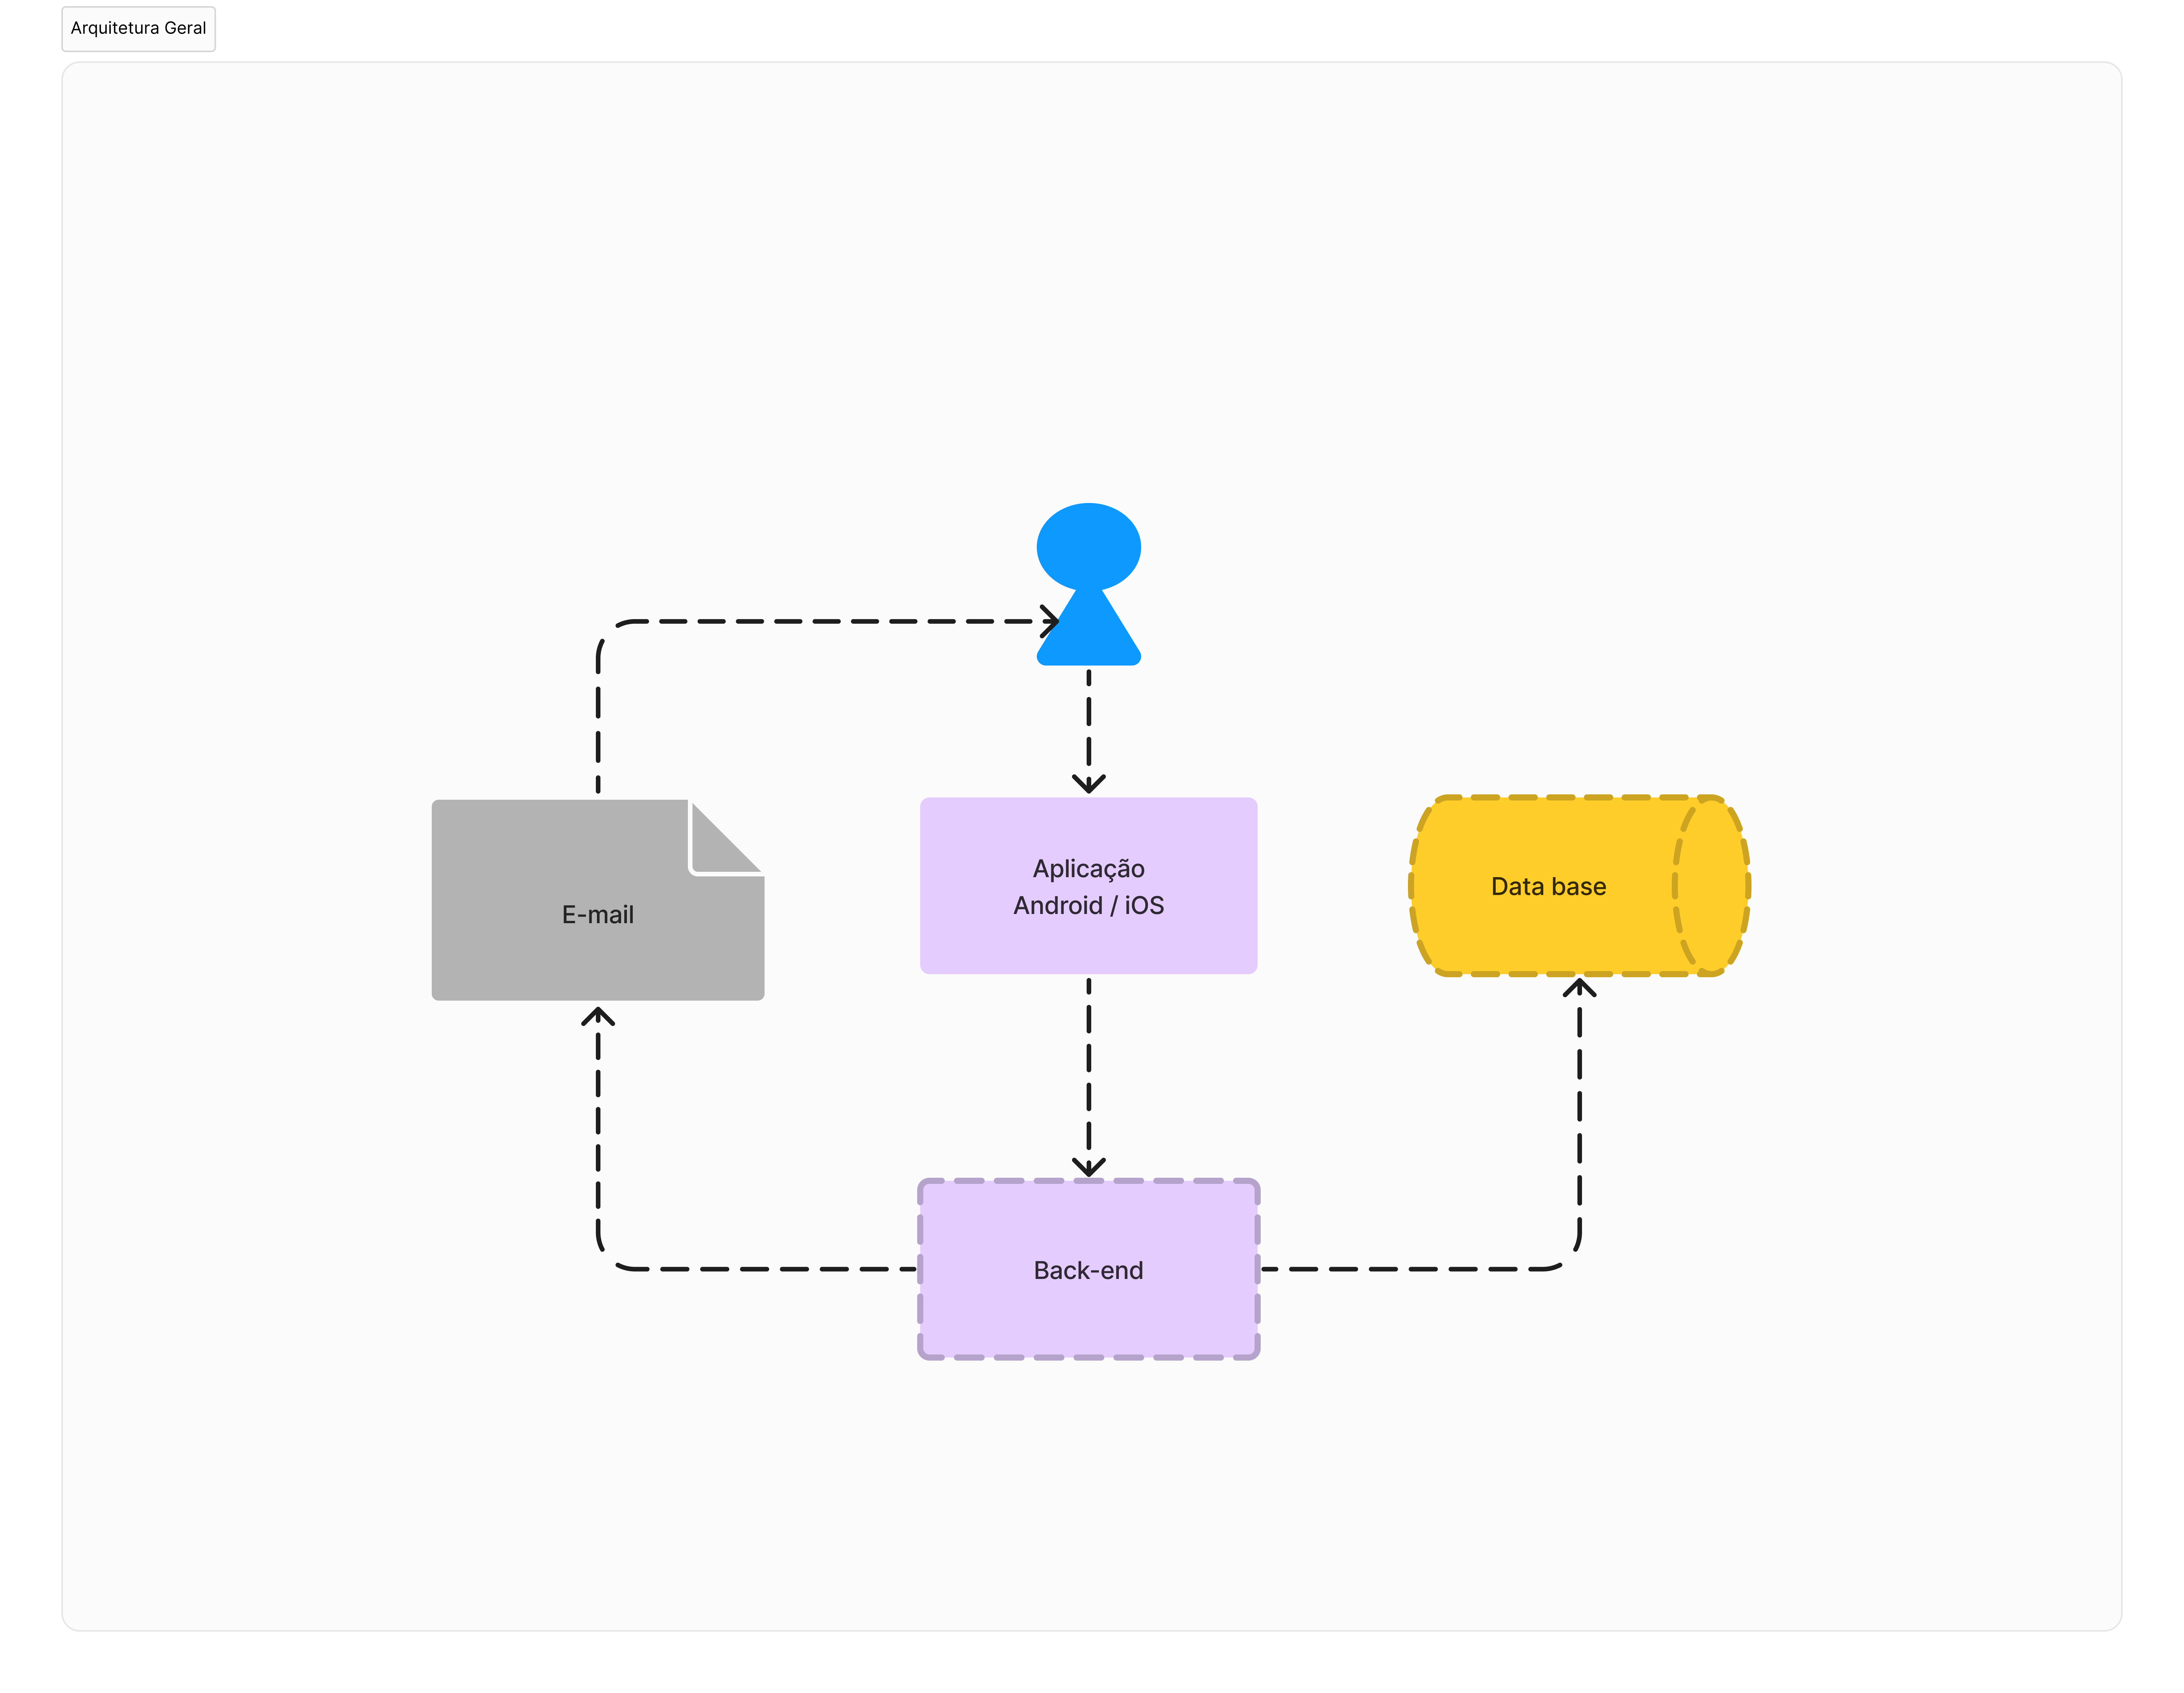
\includegraphics[scale=0.17]{figs/arq_geral.png}
            \captionof{figure}{Arquitetura de Software}
            \label{fig:arq-geral}
        \end{minipage}
    \end{center}

A figura 13 abaixo contém a arquitetura específica do sistema.

    \vspace{\baselineskip}
    \begin{center}
        \begin{minipage}{\textwidth}
            \centering
            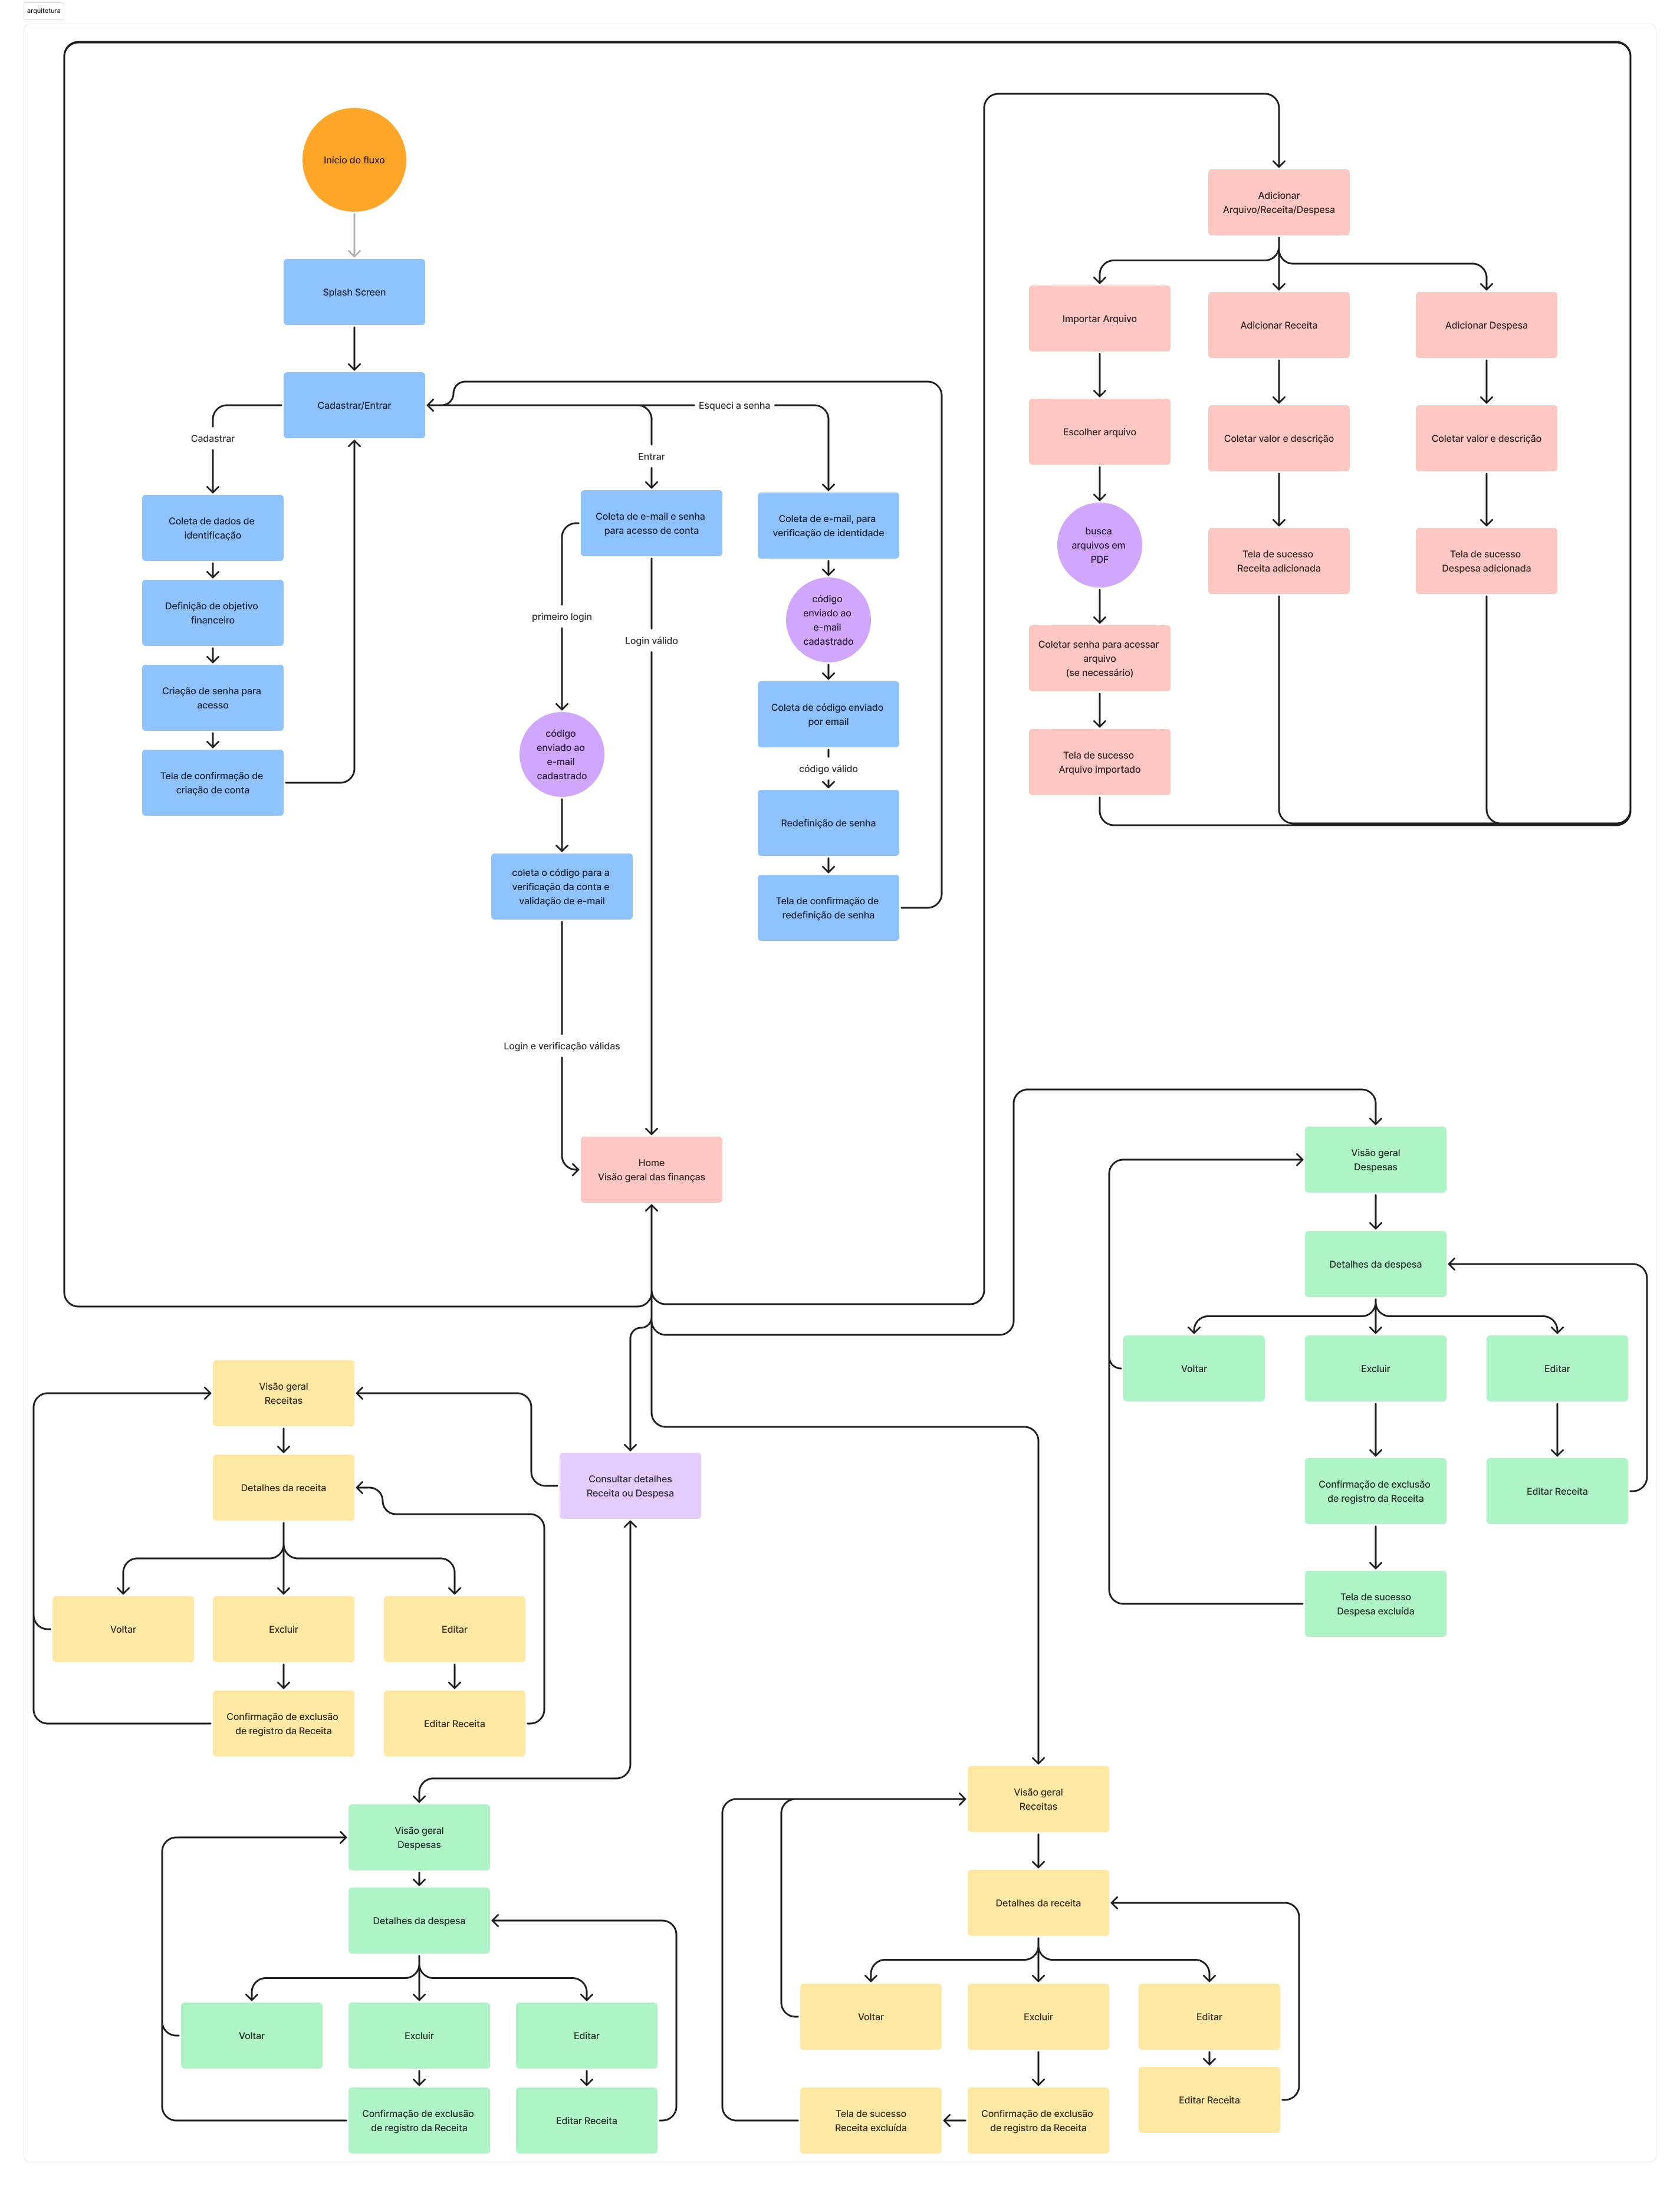
\includegraphics[scale=0.08]{figs/figura13.png}
            \captionof{figure}{Arquitetura Específica do Sistema}
            \label{fig:figura13}
        \end{minipage}
    \end{center}

\section{Desenho do Projeto de Banco de Dados}

Na figura 14 é apresentado o desenho do projeto do banco de dados.

    \vspace{\baselineskip}
    \begin{center}
        \begin{minipage}{\textwidth}
            \centering
            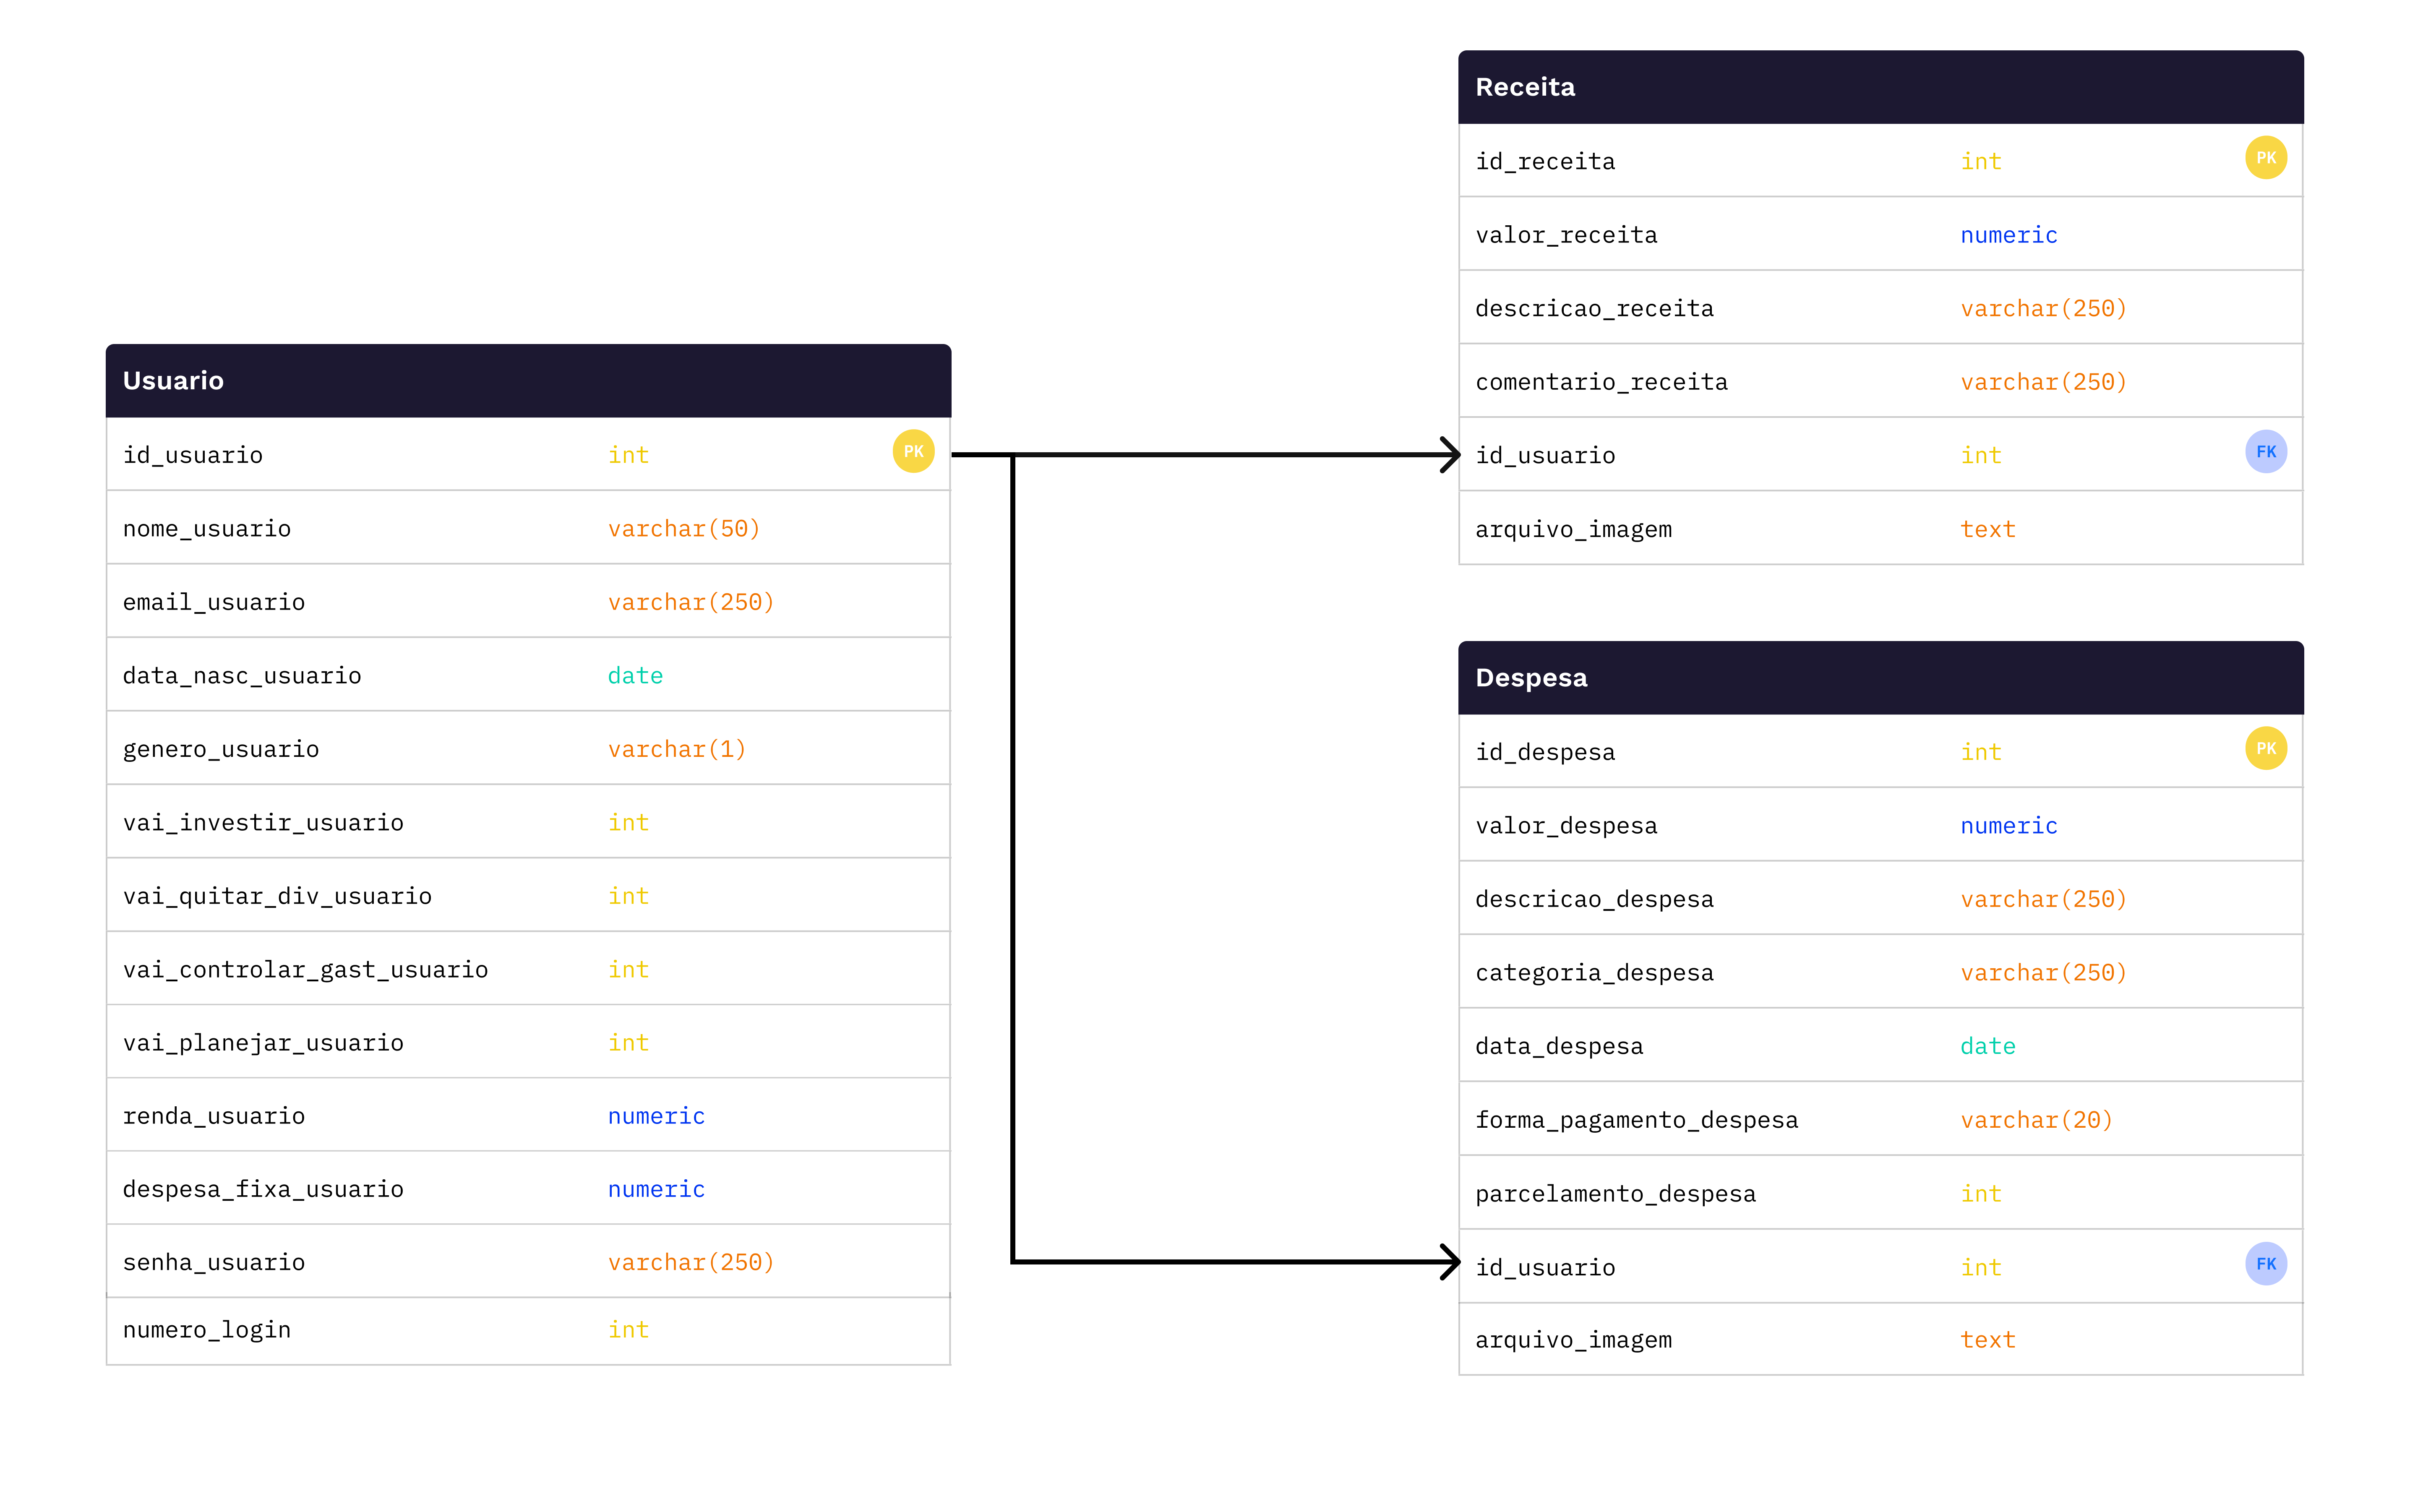
\includegraphics[scale=0.18]{figs/uml.png}
            \captionof{figure}{Desenho do Projeto do Banco de Dados}
            \label{fig:uml}
        \end{minipage}
    \end{center}

\section{Dicionário Básico do Banco de Dados}

    A tabela 1 corresponde ao dicionário da tabela 'usuario'.

\begin{table}[ht]
    \centering
    \setlength{\extrarowheight}{3pt}  % Aumenta a altura das linhas da tabela

    \begin{center}
        \begin{minipage}{\textwidth}
            \centering
            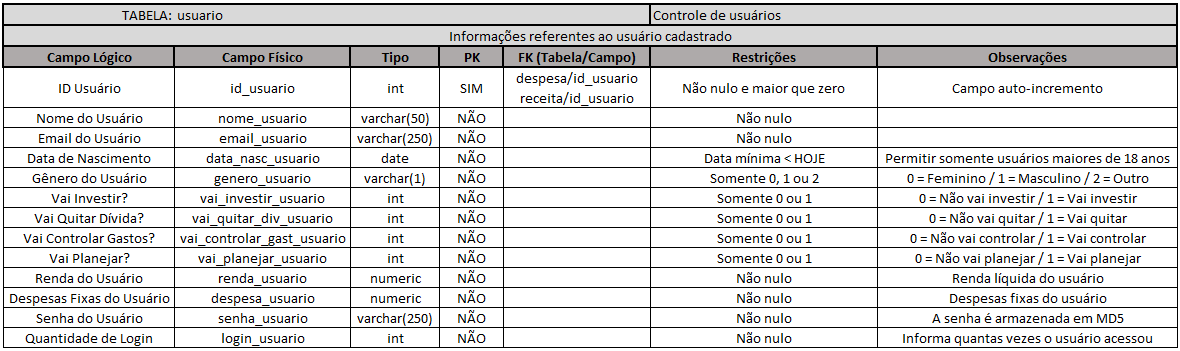
\includegraphics[scale=0.5]{figs/tab1.png}
        \end{minipage}
    \end{center}

    \caption{Dicionário da Tabela de Usuário}
    \label{tab:tab1}
\end{table}


    A tabela 2 corresponde ao dicionário da tabela 'despesa'.

\begin{table}[ht]
    \centering
    \setlength{\extrarowheight}{3pt}  % Aumenta a altura das linhas da tabela

    \begin{center}
        \begin{minipage}{\textwidth}
            \centering
            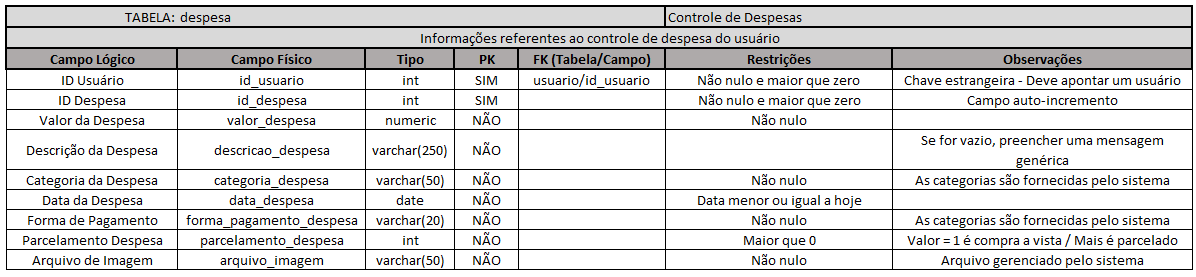
\includegraphics[scale=0.5]{figs/tab2.png}
        \end{minipage}
    \end{center}

    \caption{Dicionário da Tabela de Despesas}
    \label{tab:tab1}
\end{table}

    A tabela 3 corresponde ao dicionário da tabela 'receita'.

\begin{table}[ht]
    \centering
    \setlength{\extrarowheight}{3pt}  % Aumenta a altura das linhas da tabela

    \begin{center}
        \begin{minipage}{\textwidth}
            \centering
            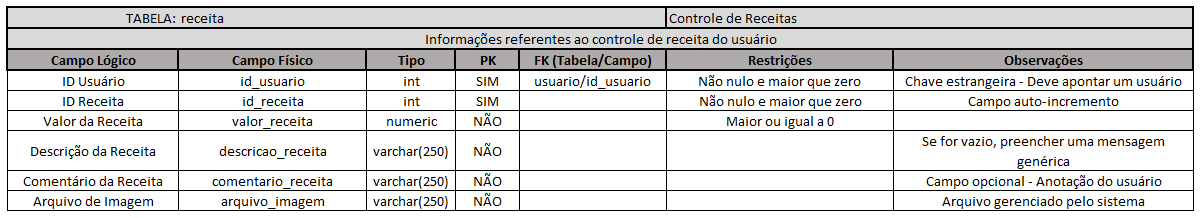
\includegraphics[scale=0.5]{figs/tab3.png}
        \end{minipage}
    \end{center}

    \caption{Dicionário da Tabela de Receitas}
    \label{tab:tab1}
\end{table}

\vspace{\baselineskip}
\vspace{\baselineskip}
\vspace{\baselineskip}

\section{Implementação}

Nesta seção do projeto serão apresentadas as principais telas desenvolvidas do \textit{Front End}.

\subsection{Tela de Login}

Esta é a tela inicial do aplicativo, onde todos os usuários poderão acessar utilizando um endereço de \textit{e-mail} e senha previamente cadastrados. Caso seja a primeira vez que o usuário está utilizando o aplicativo, será necessário realizar um cadastro clicando no botão \textbf{"Cadastrar"} conforme descrito na figura 15.

    \vspace{\baselineskip}
    \begin{center}
        \begin{minipage}{\textwidth}
            \centering
            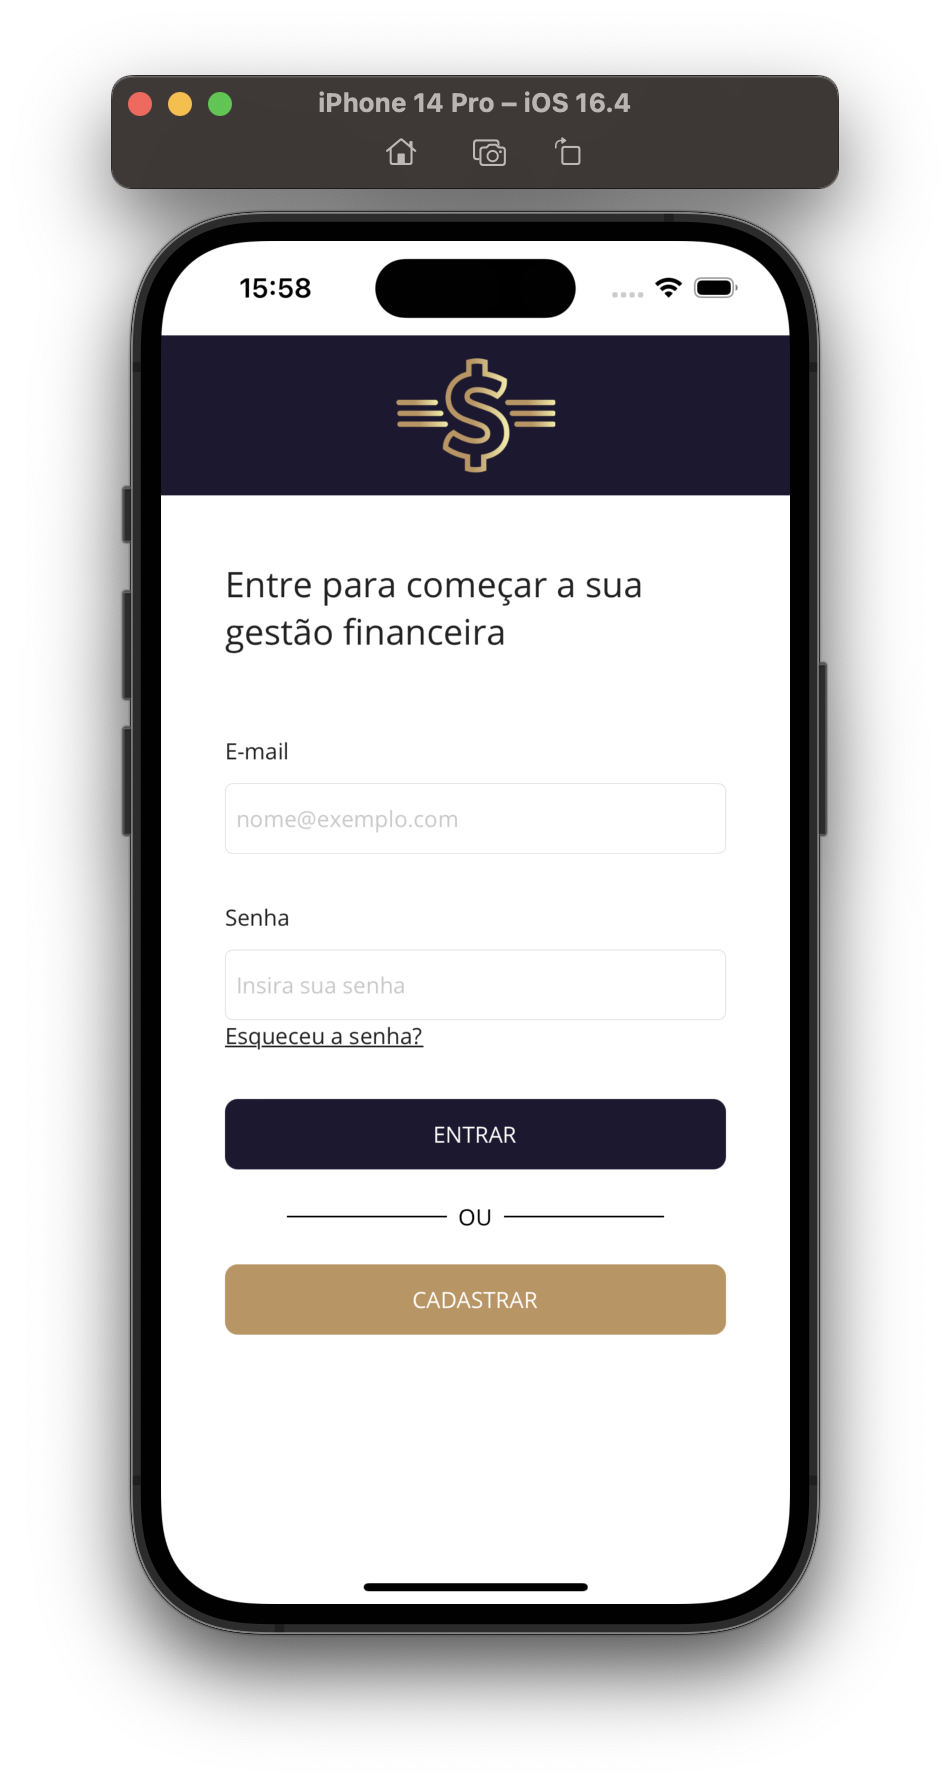
\includegraphics[scale=0.17]{figs/figura15.png}
            \captionof{figure}{Página de Login}
            \label{fig:uml}
        \end{minipage}
    \end{center}    

\subsection{Cadastro}

Conforme figura 16, para que o usuário possa realizar o cadastro, serão necessárias algumas informações, tais como: nome completo, \textit{e-mail}, data de nascimento e o gênero. Ao preencher todas as informações solicitadas, basta clicar no botão \textbf{“Próximo”}.

    \begin{center}
        \begin{minipage}{0.3\textwidth}
            \centering
            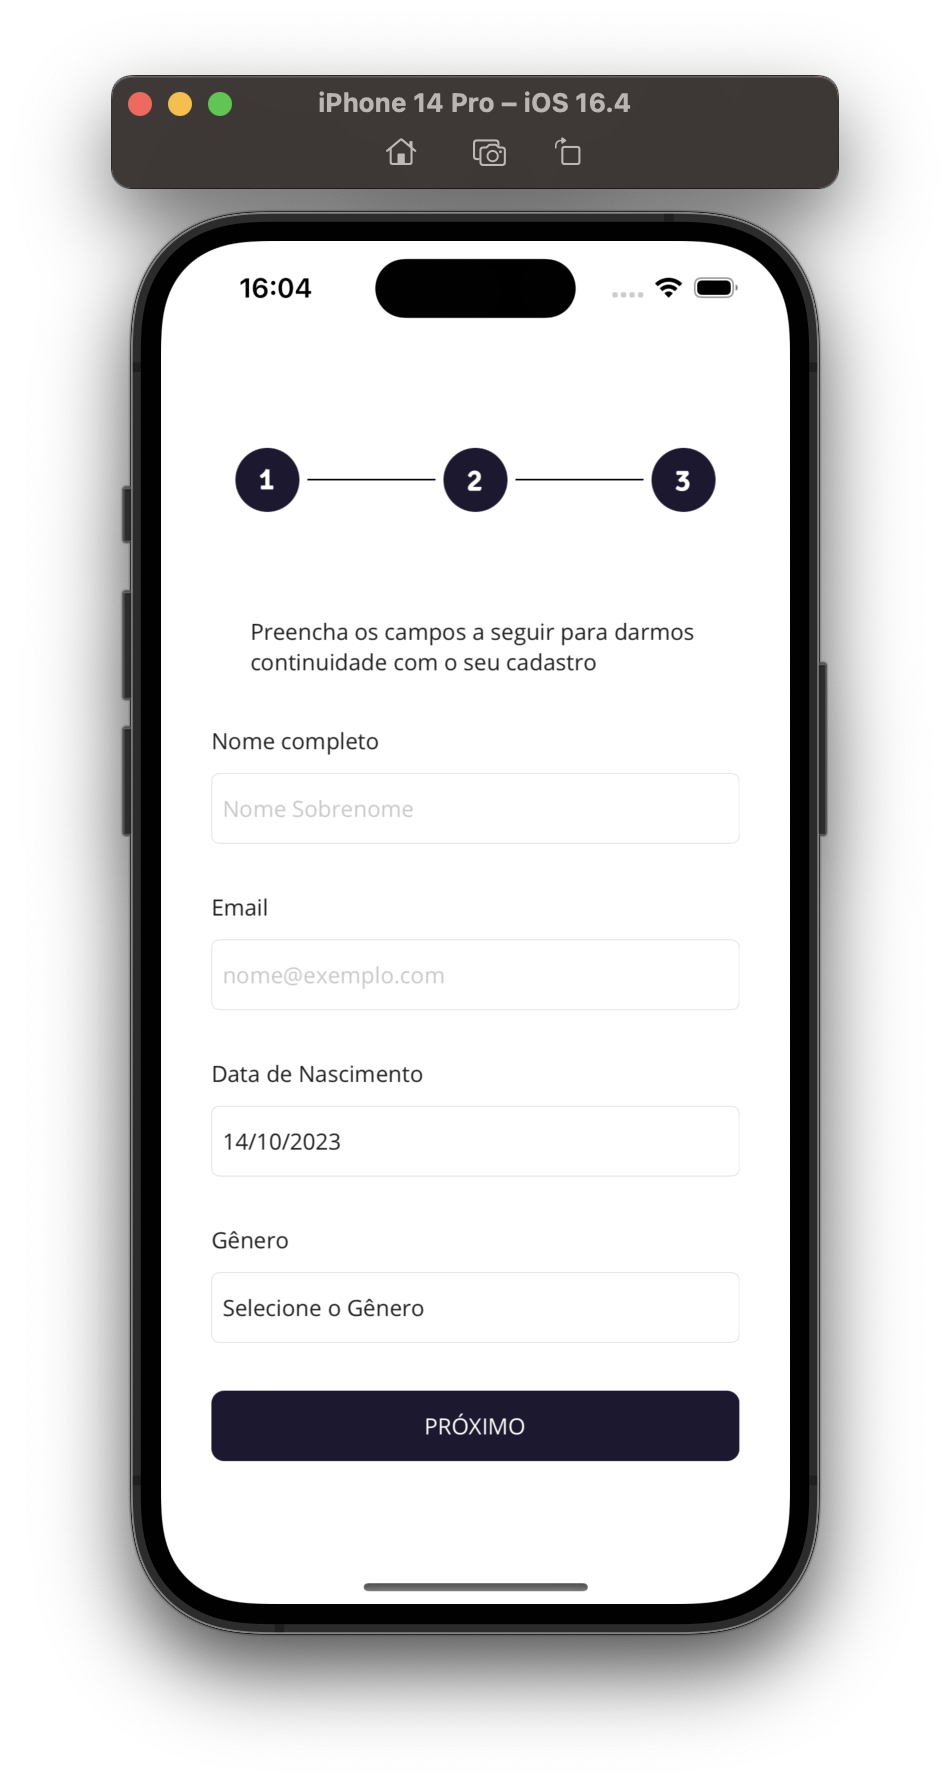
\includegraphics[scale=0.17]{figs/figura16.png}
            \captionof{figure}{Cadastro I}
            \label{fig:figura16}
        \end{minipage}%
    \end{center}
    

Conforme figura 17, uma nova tela aparecerá contendo alguns objetivos, bem como a média mensal de renda e despesas, a fim de entendermos melhor o perfil do usuário. Após preencher todos os campos obrigatórios, clique no botão \textbf{“Próximo”}.

    \begin{center}
        \begin{minipage}{0.3\textwidth}
            \centering
            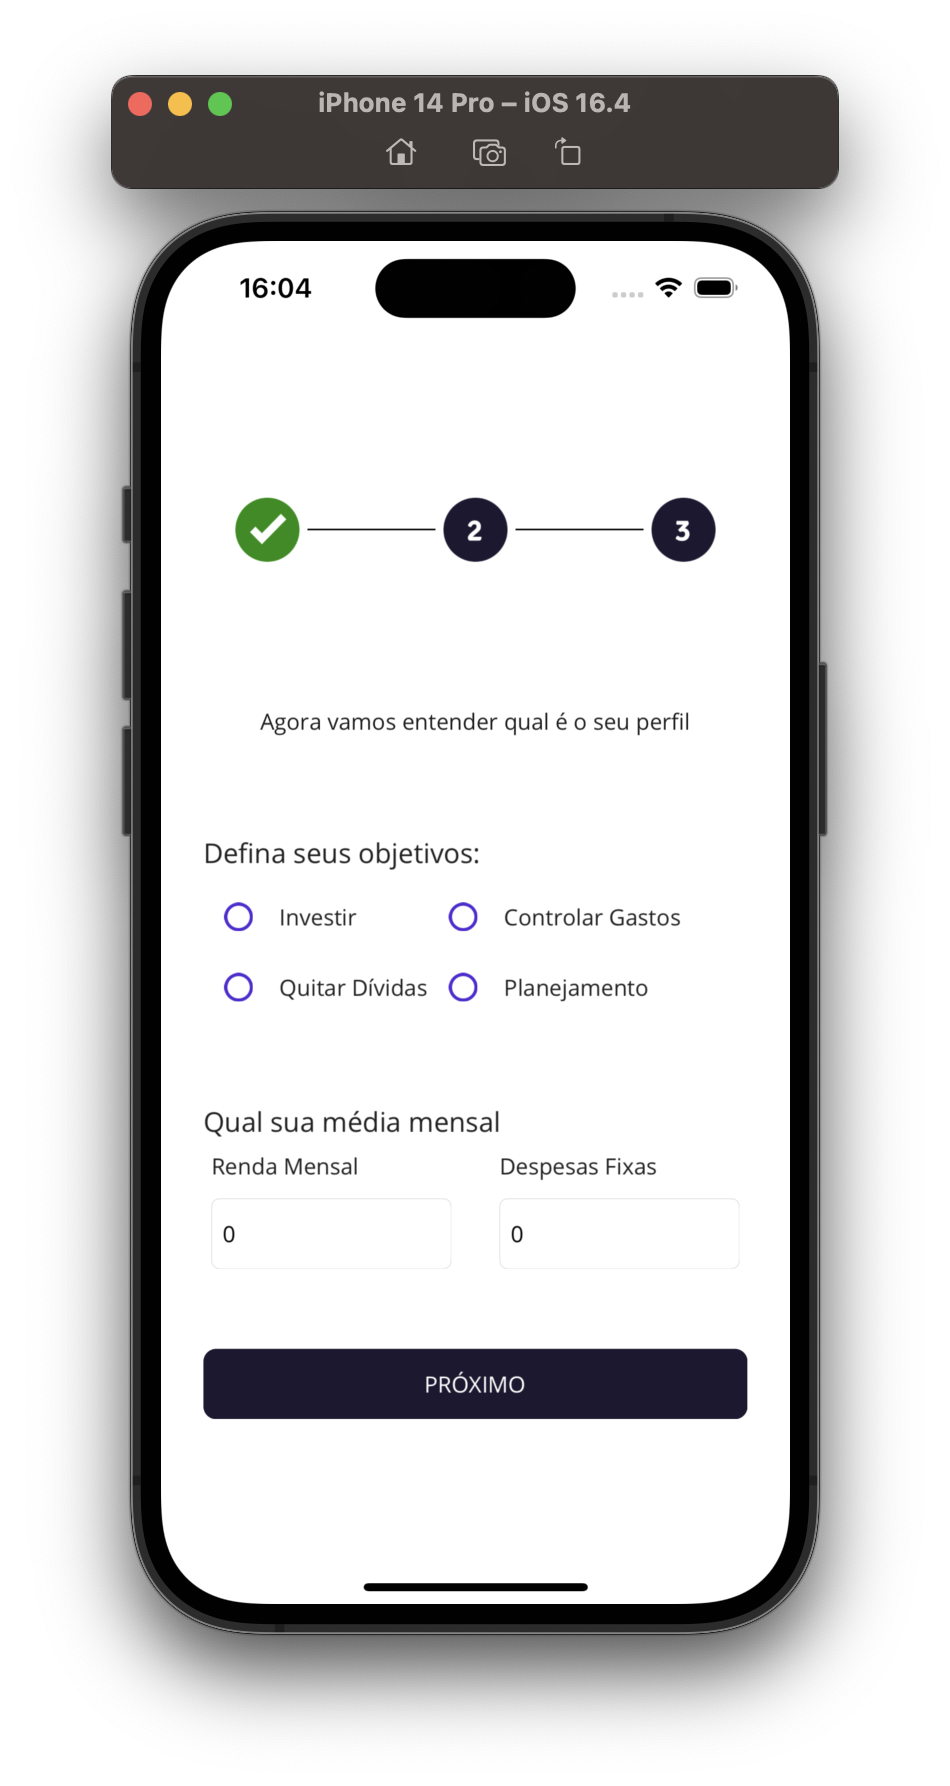
\includegraphics[scale=0.2]{figs/figura17.png}
            \captionof{figure}{Cadastro II}
            \label{fig:figura17}
        \end{minipage}%
    \end{center}

Conforme figura 18, aparecerá uma última tela destinada à criação de senha. Algumas especificações são de extrema importância para garantir a segurança dos dados do usuário. A senha deve conter no mínimo 8 caracteres, incluindo ao menos um número, uma letra maiúscula e uma letra minúscula. Repita a senha para verificar se digitou corretamente e, para finalizar, clique no botão \textbf{“Próximo”}. 

    \begin{center}
        \begin{minipage}{0.3\textwidth}
            \centering
            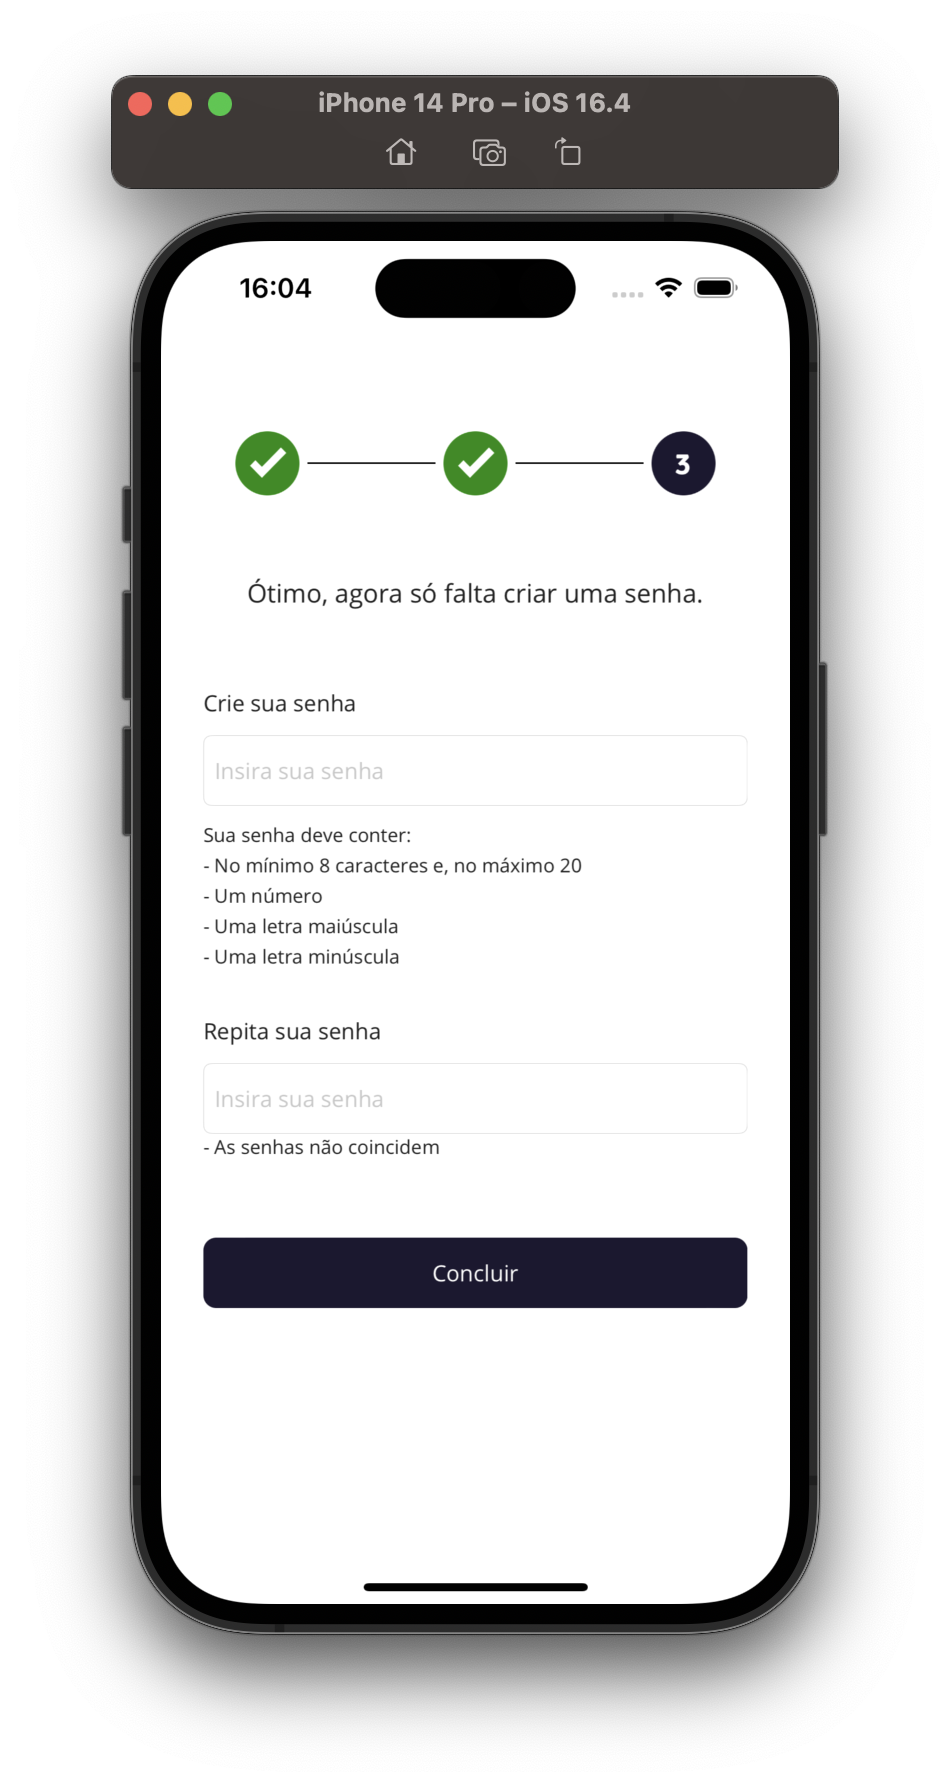
\includegraphics[scale=0.2]{figs/figura18.png}
            \captionof{figure}{Cadastro III}
            \label{fig:figura18}
        \end{minipage}%
    \end{center}

\vspace{\baselineskip}
\vspace{\baselineskip}
\vspace{\baselineskip}
\vspace{\baselineskip}
\vspace{\baselineskip}
\vspace{\baselineskip}

Na figura 19 apresentada, uma nova tela será exibida apenas para confirmar que o cadastro foi concluído com sucesso.

    \vspace{\baselineskip}
    \begin{center}
        \begin{minipage}{\textwidth}
            \centering
            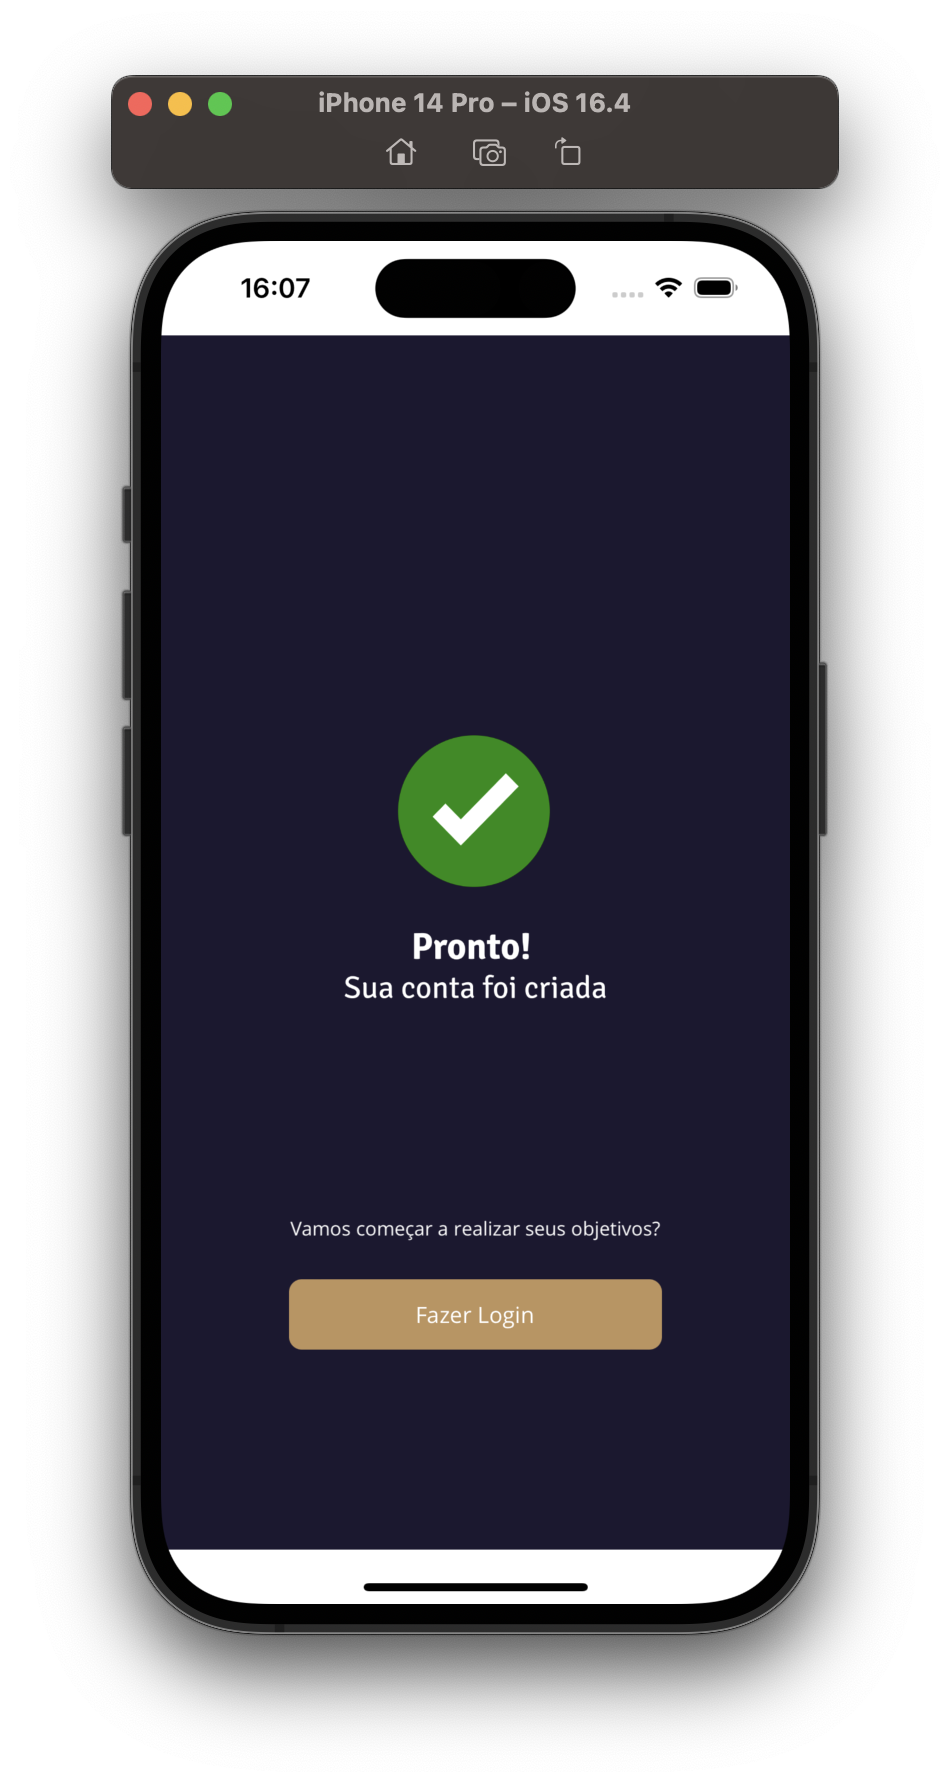
\includegraphics[scale=0.2]{figs/figura19.png}
            \captionof{figure}{Conta Criada}
            \label{fig:figura19}
        \end{minipage}
    \end{center}  
    
\subsection{Menu Principal}

Na figura 20 é descrito o menu principal

    \vspace{\baselineskip}
    \begin{center}
        \begin{minipage}{\textwidth}
            \centering
            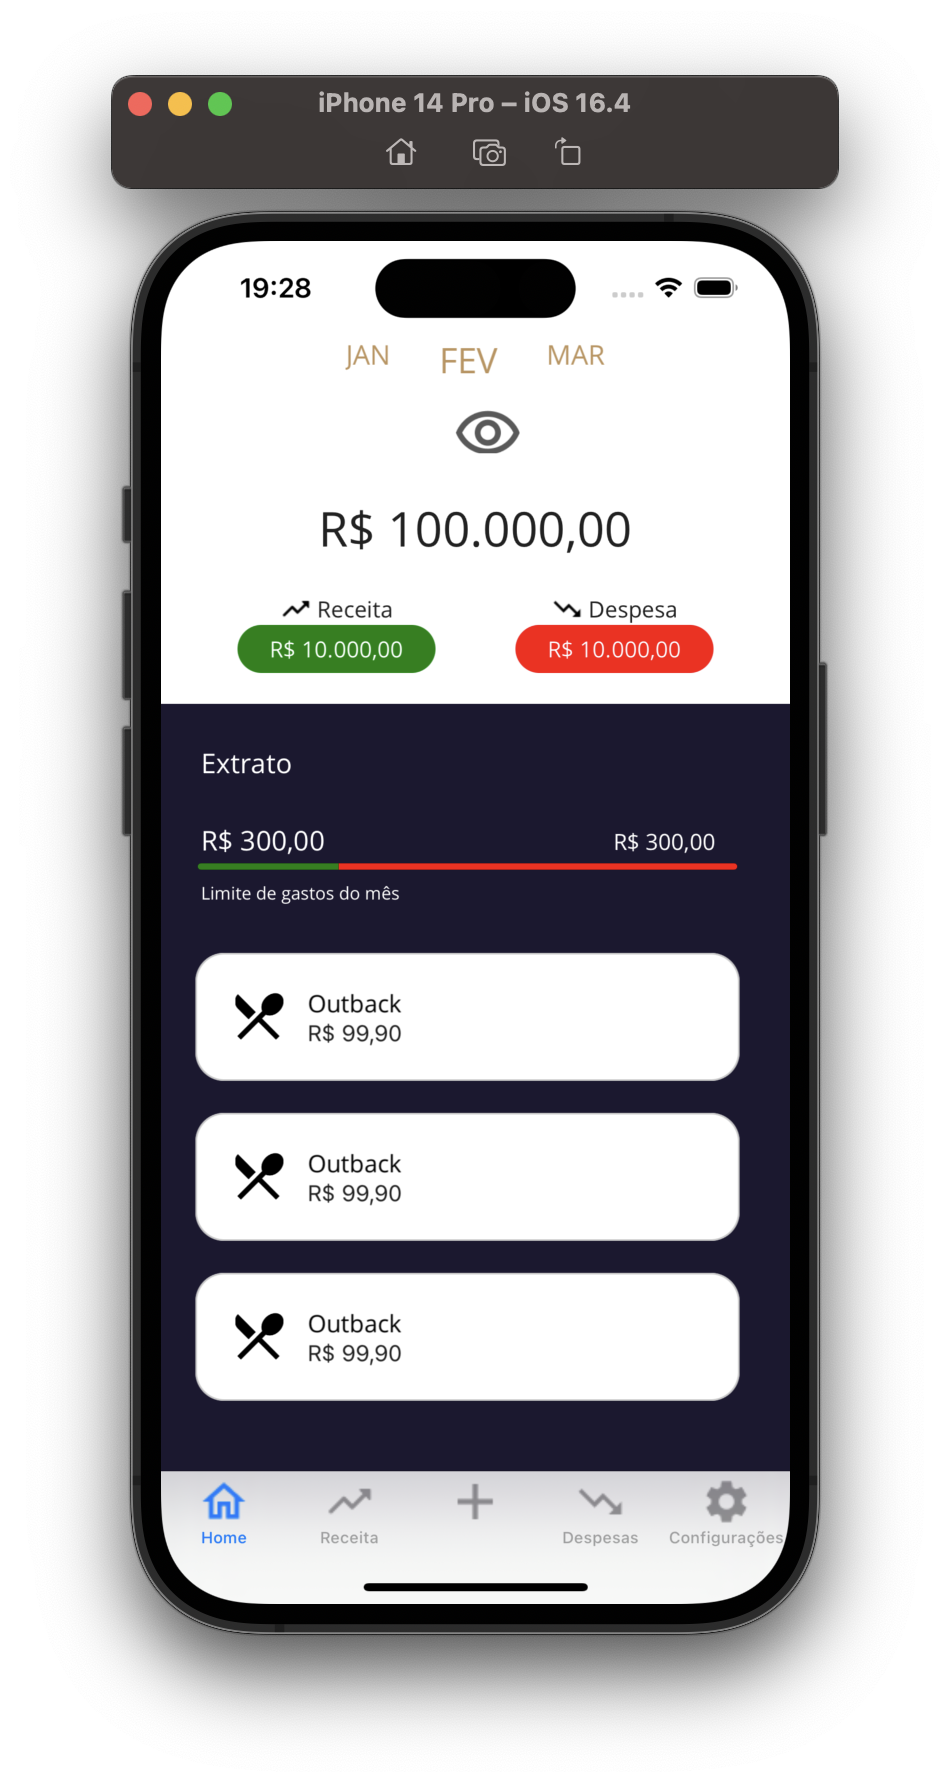
\includegraphics[scale=0.2]{figs/fig20.png}
            \captionof{figure}{Menu Principal}
            \label{fig:figura20}
        \end{minipage}
    \end{center}  

Após fazer o login, é possível utilizar o aplicativo, a imagem acima representa o menu principal, ou também bastante conhecida como \textit{“home”}, contendo diversas opções, tais como: saldo disponível, receita, despesas, extrato e alguns botões na parte inferior da tela. Além disso na parte superior da tela é possível ver informações referentes a meses passados e ou futuros. 

\subsection{Menu Principal com Informações Escondidas}

Na figura 21 é descrito o menu principal com informações escondidas.

    \vspace{\baselineskip}
    \begin{center}
        \begin{minipage}{\textwidth}
            \centering
            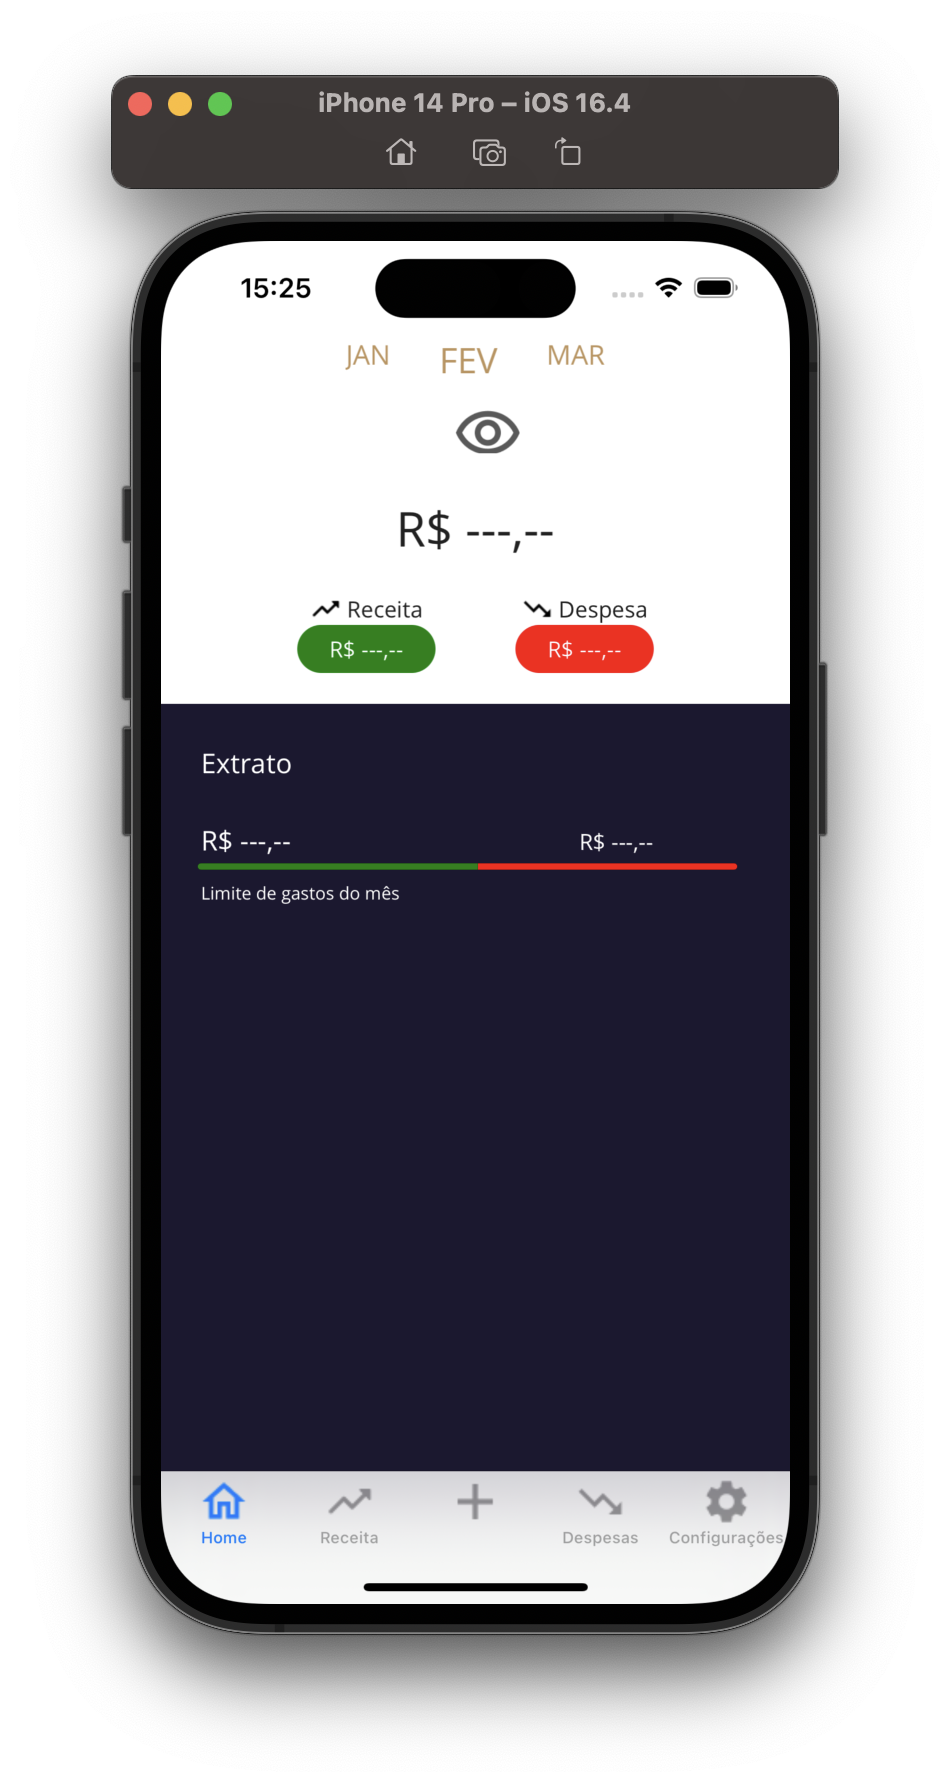
\includegraphics[scale=0.2]{figs/figura21.png}
            \captionof{figure}{Menu Principal com Informações Escondidas}
            \label{fig:figura21}
        \end{minipage}
    \end{center}  

Há a possibilidade de esconder informações que o usuário não queira exibir, como o saldo, o valor do extrato, a receita e as despesas. Essas informações são apresentadas na figura 22.

    \vspace{\baselineskip}
    \begin{center}
        \begin{minipage}{\textwidth}
            \centering
            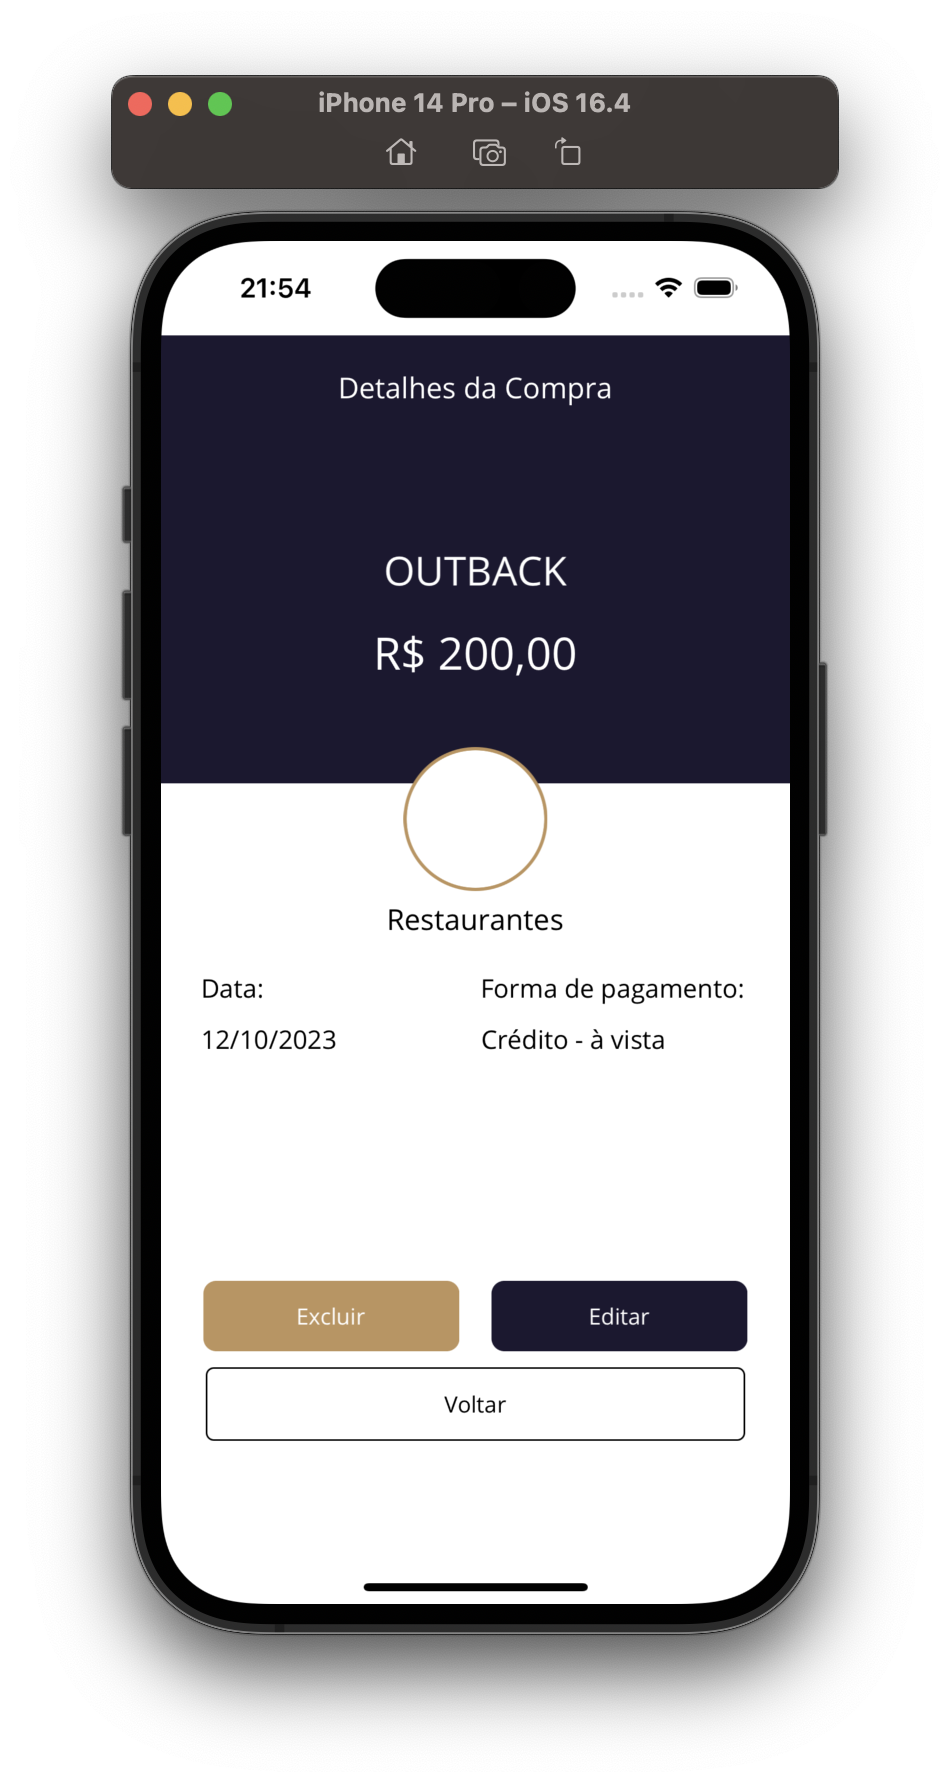
\includegraphics[scale=0.2]{figs/fig22.png}
            \captionof{figure}{Extrato com Informações}
            \label{fig:figura22}
        \end{minipage}
    \end{center}  

No extrato será possível visualizar um gasto detalhadamente, incluindo a data e hora da compra, numeração final do cartão utilizado e a opção de relatar uma compra que o cliente considerar não ter sido feita por ele. 

Conforme a figura 23, é possível notar que temos três opções clicando nesse botão central de \textbf{“+”}, onde, cada uma dessas opções significa uma funcionalidade diferente. A primeira opção é \textbf{“Importar PDF”} que será explicado logo abaixo. A segunda e a terceira opção são voltadas a adicionar algo que seria receita e despesa respectivamente. 

    \vspace{\baselineskip}
    \begin{center}
        \begin{minipage}{\textwidth}
            \centering
            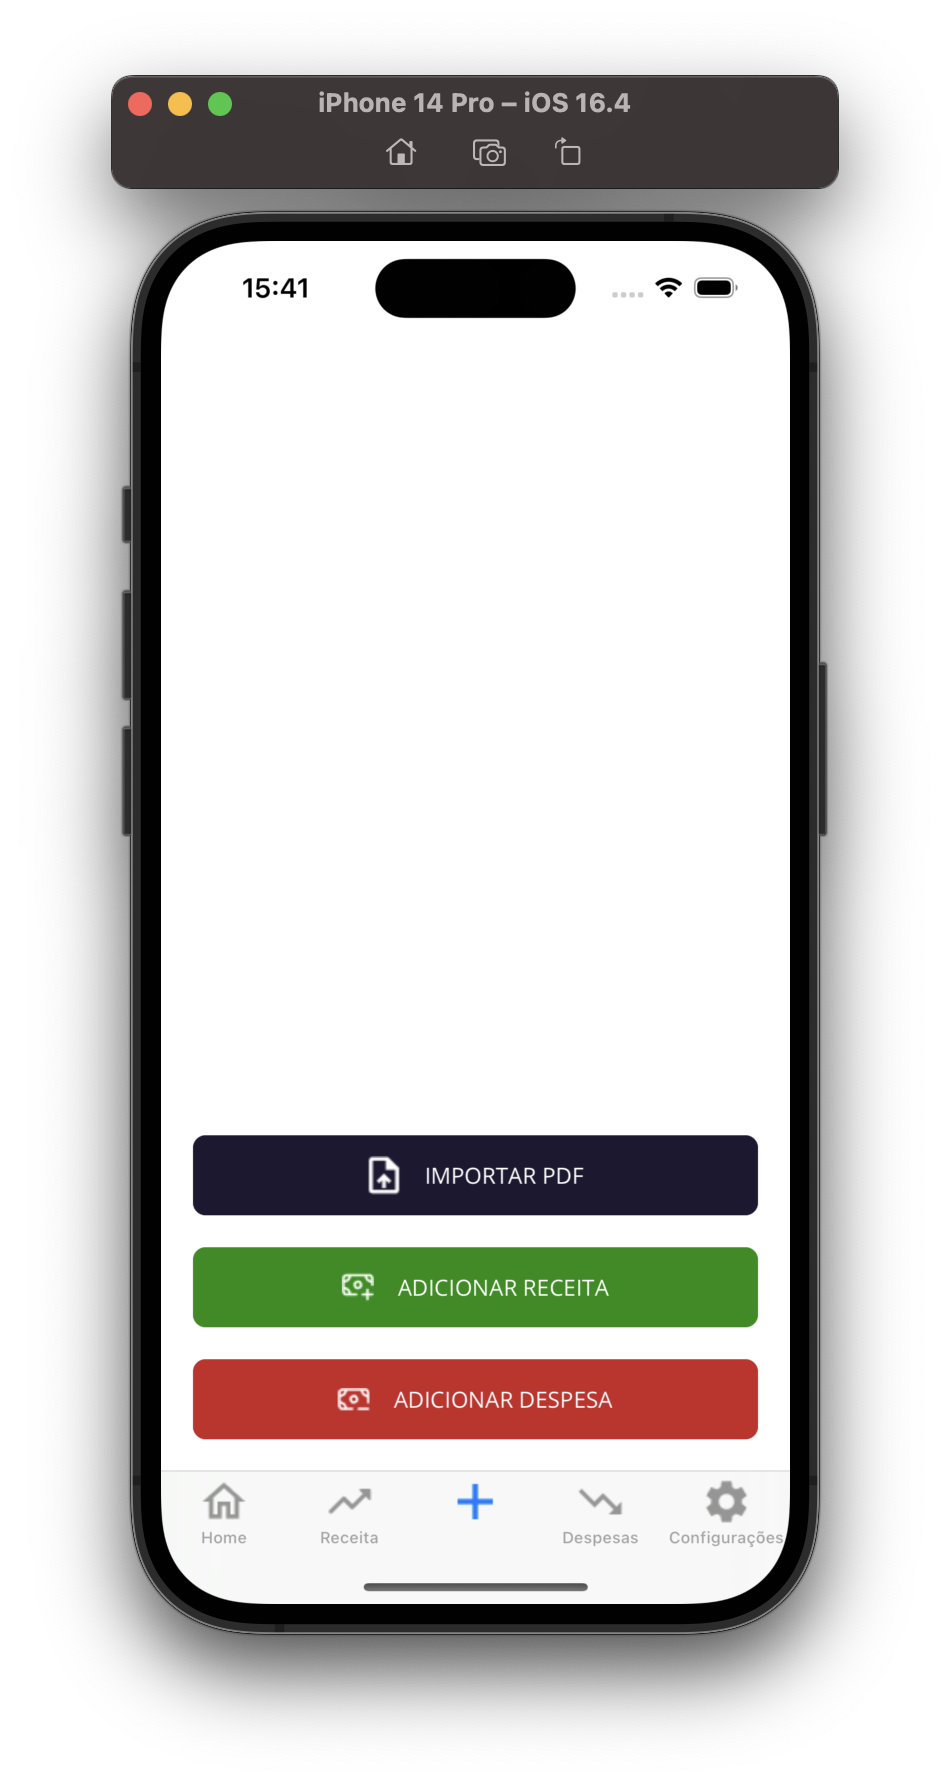
\includegraphics[scale=0.2]{figs/figura23.png}
            \captionof{figure}{Menu com Três Opções}
            \label{fig:figura23}
        \end{minipage}
    \end{center}     

Ao clicar na opção de \textbf{“Importar PDF”} uma nova tela para a importação de PDF aparecerá, assim como mostrado na figura 24. Nessa aba de importação de PDF, temos como campos a escolha do PDF a ser importado. Caso seja necessária uma senha para acessar o arquivo, basta clicar no botão \textbf{“Sim”} e imediatamente abaixo, o campo para digitar a senha será habilitado. Se não for necessária uma senha, selecione o botão \textbf{“Não”} que o campo abaixo permanecerá desativado. Ao finalizar clicar no botão \textbf{“Importar Arquivo”}, após clicar uma nova tela aparecerá indicando sucesso na operação, conforme figura 25. 

    \vspace{\baselineskip}
    \begin{center}
        \begin{minipage}{0.4\textwidth}
            \centering
            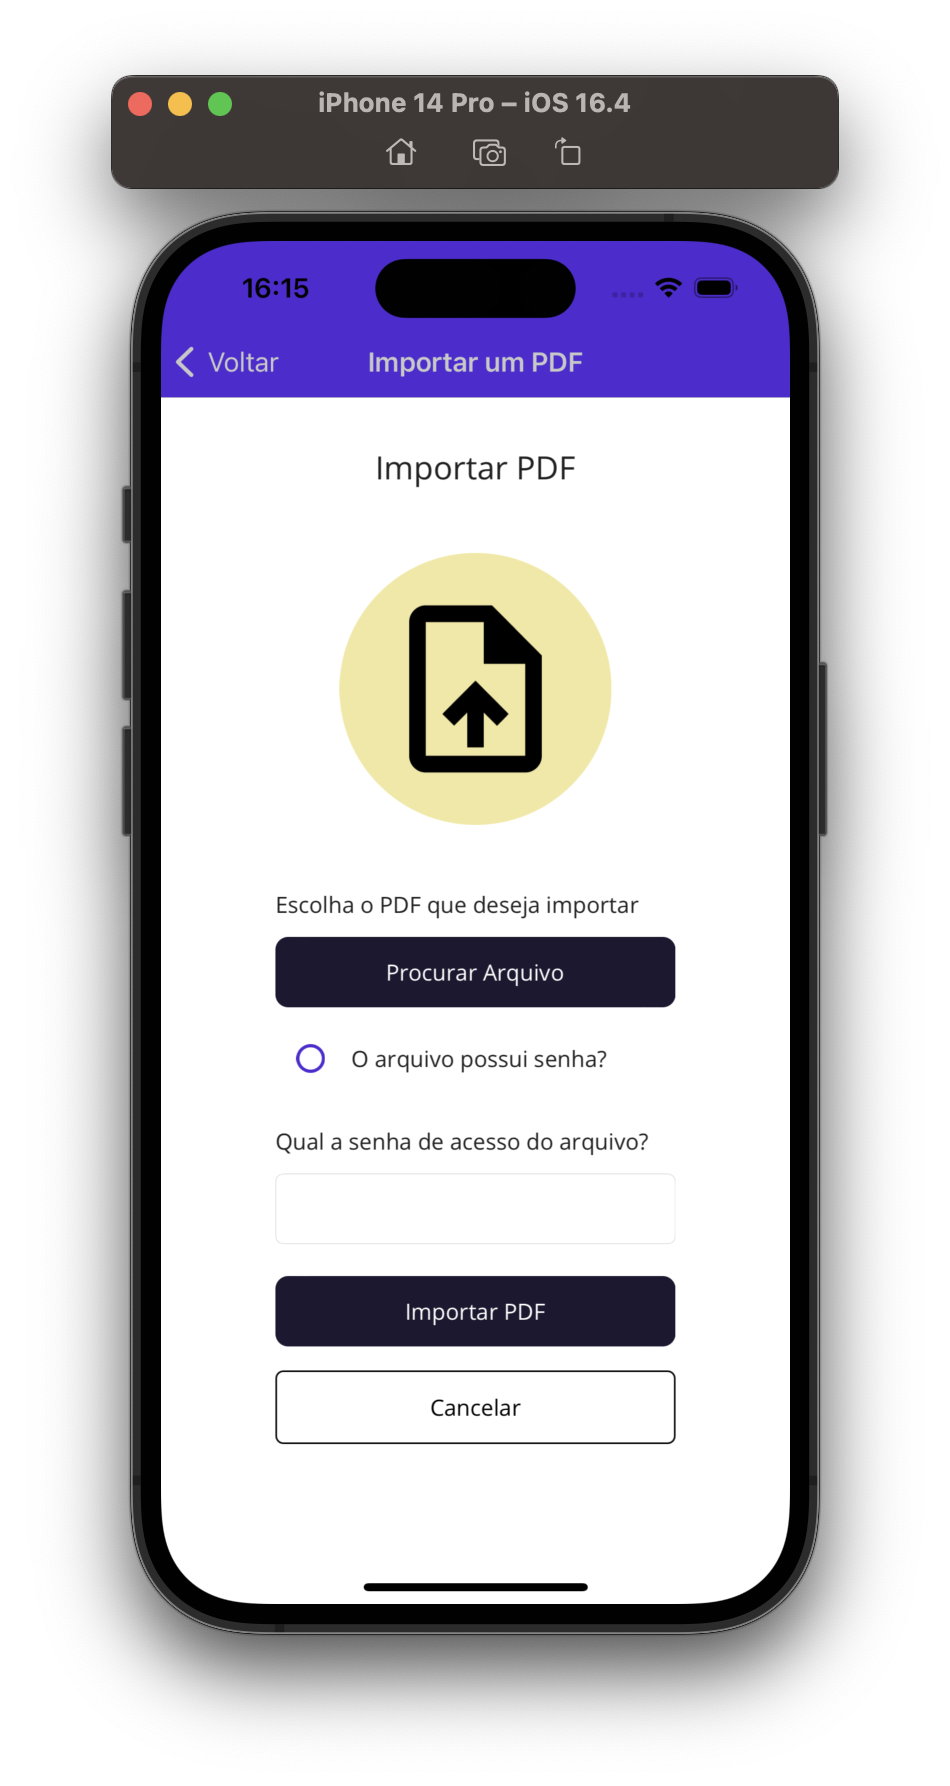
\includegraphics[scale=0.2]{figs/figura24.png}
            \captionof{figure}{Importar PDF I}
            \label{fig:figura24}
        \end{minipage}%
        \begin{minipage}{0.4\textwidth}
            \centering
            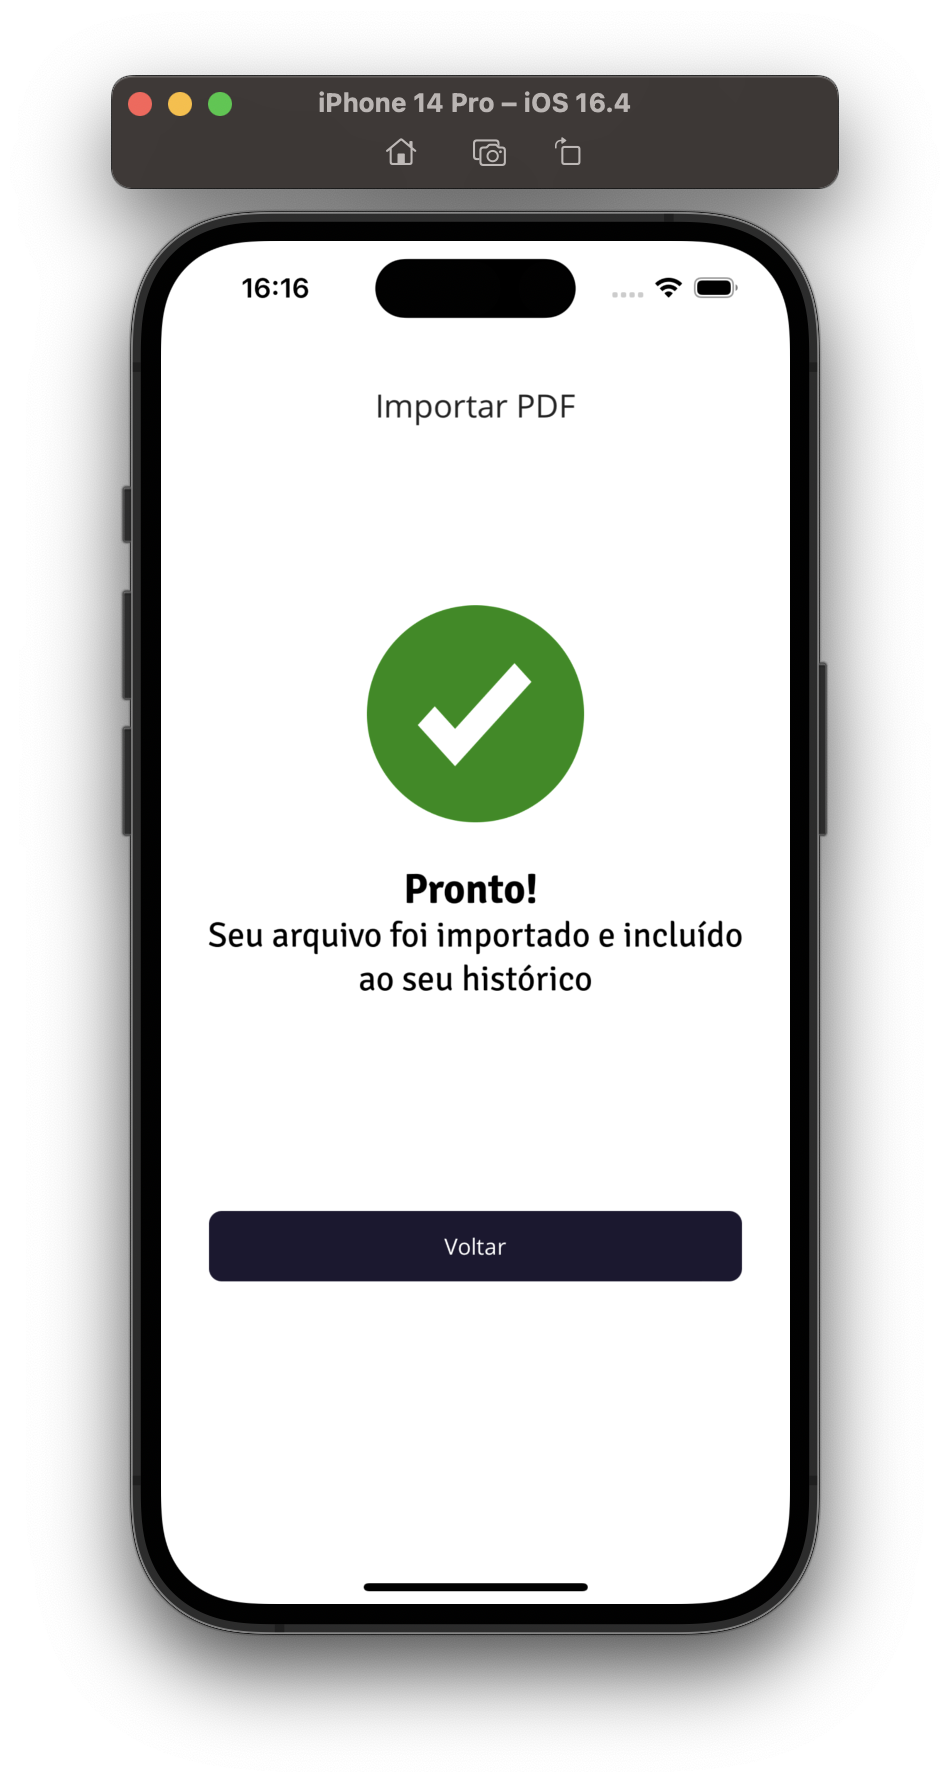
\includegraphics[scale=0.2]{figs/figura25.png}
            \captionof{figure}{Importar PDF II}
            \label{fig:figura25}
        \end{minipage}%
    \end{center}

A partir do Menu Principal ao clicar na opção \textbf{“Adicionar Receita”} aparecerá uma tela descrita na Figura 26. Nessa nova tela contém dois campos um obrigatório no qual um valor deve ser inserido, valor referente a receita. E um outro tópico não obrigatório que seria para adicionar uma descrição para essa receita. Ao preencher os devidos campos clique no botão \textbf{“Adicionar”}, e então uma tela apontando sucesso na operação aparecerá, conforme descrito na Figura 27. 

    \vspace{\baselineskip}
    \begin{center}
        \begin{minipage}{0.4\textwidth}
            \centering
            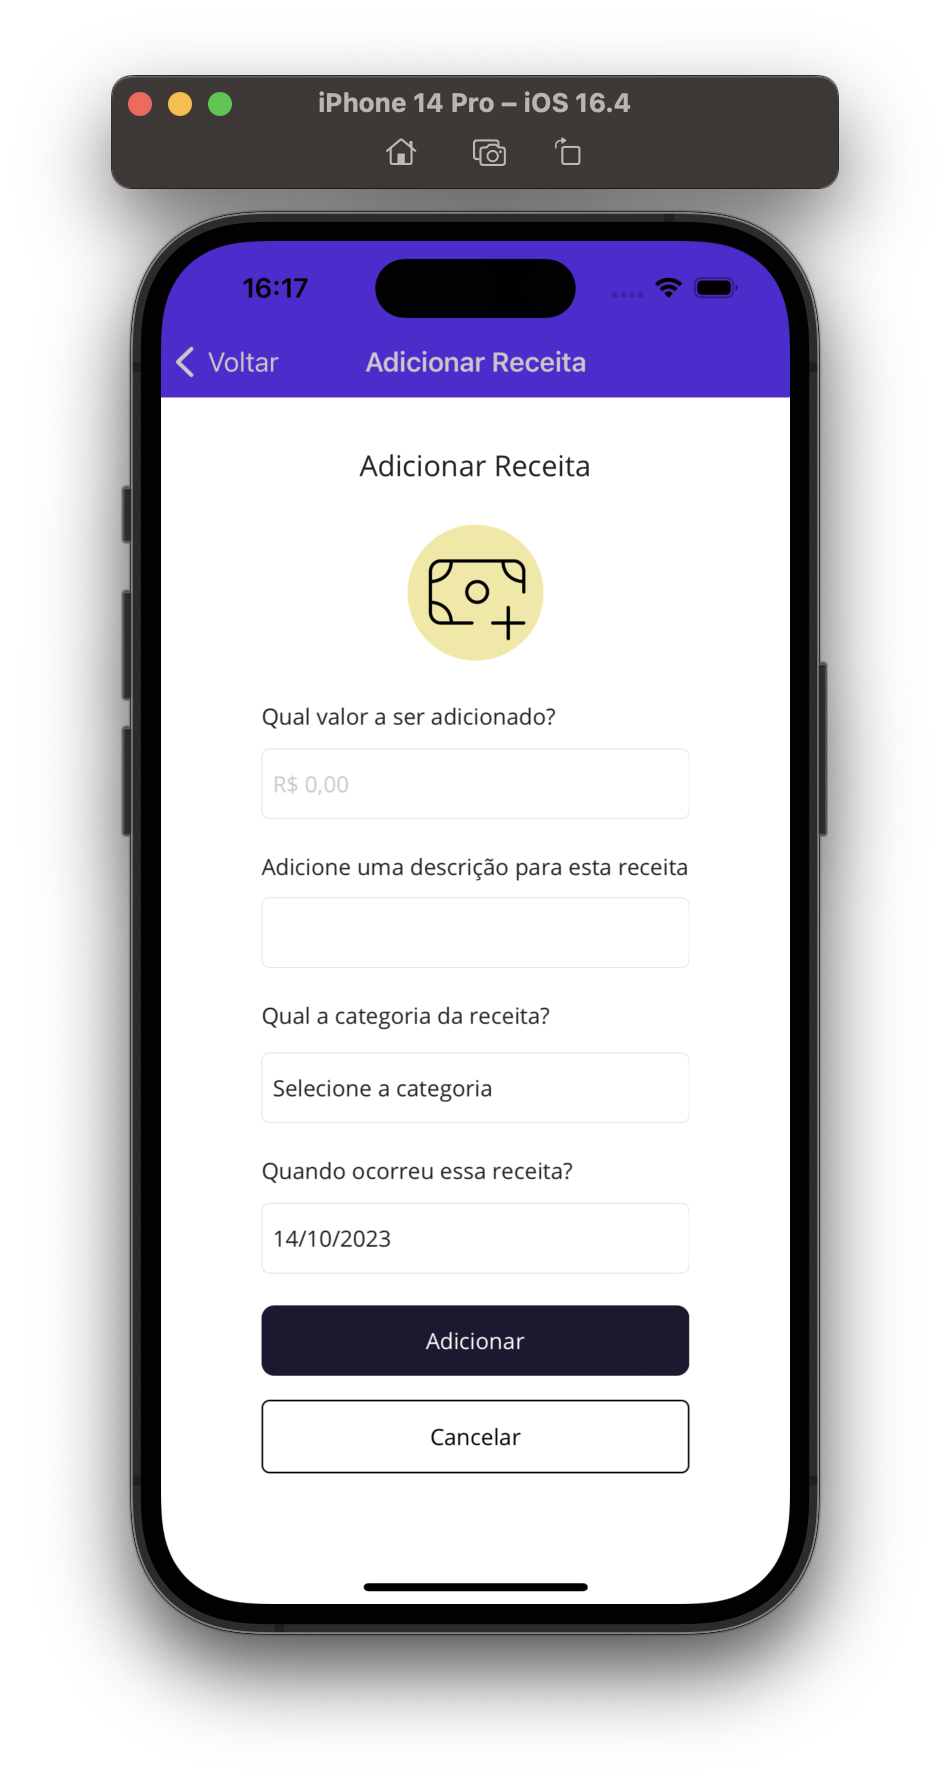
\includegraphics[scale=0.15]{figs/figura26.png}
            \captionof{figure}{Criar Receita I}
            \label{fig:figura26}
        \end{minipage}%
        \begin{minipage}{0.4\textwidth}
            \centering
            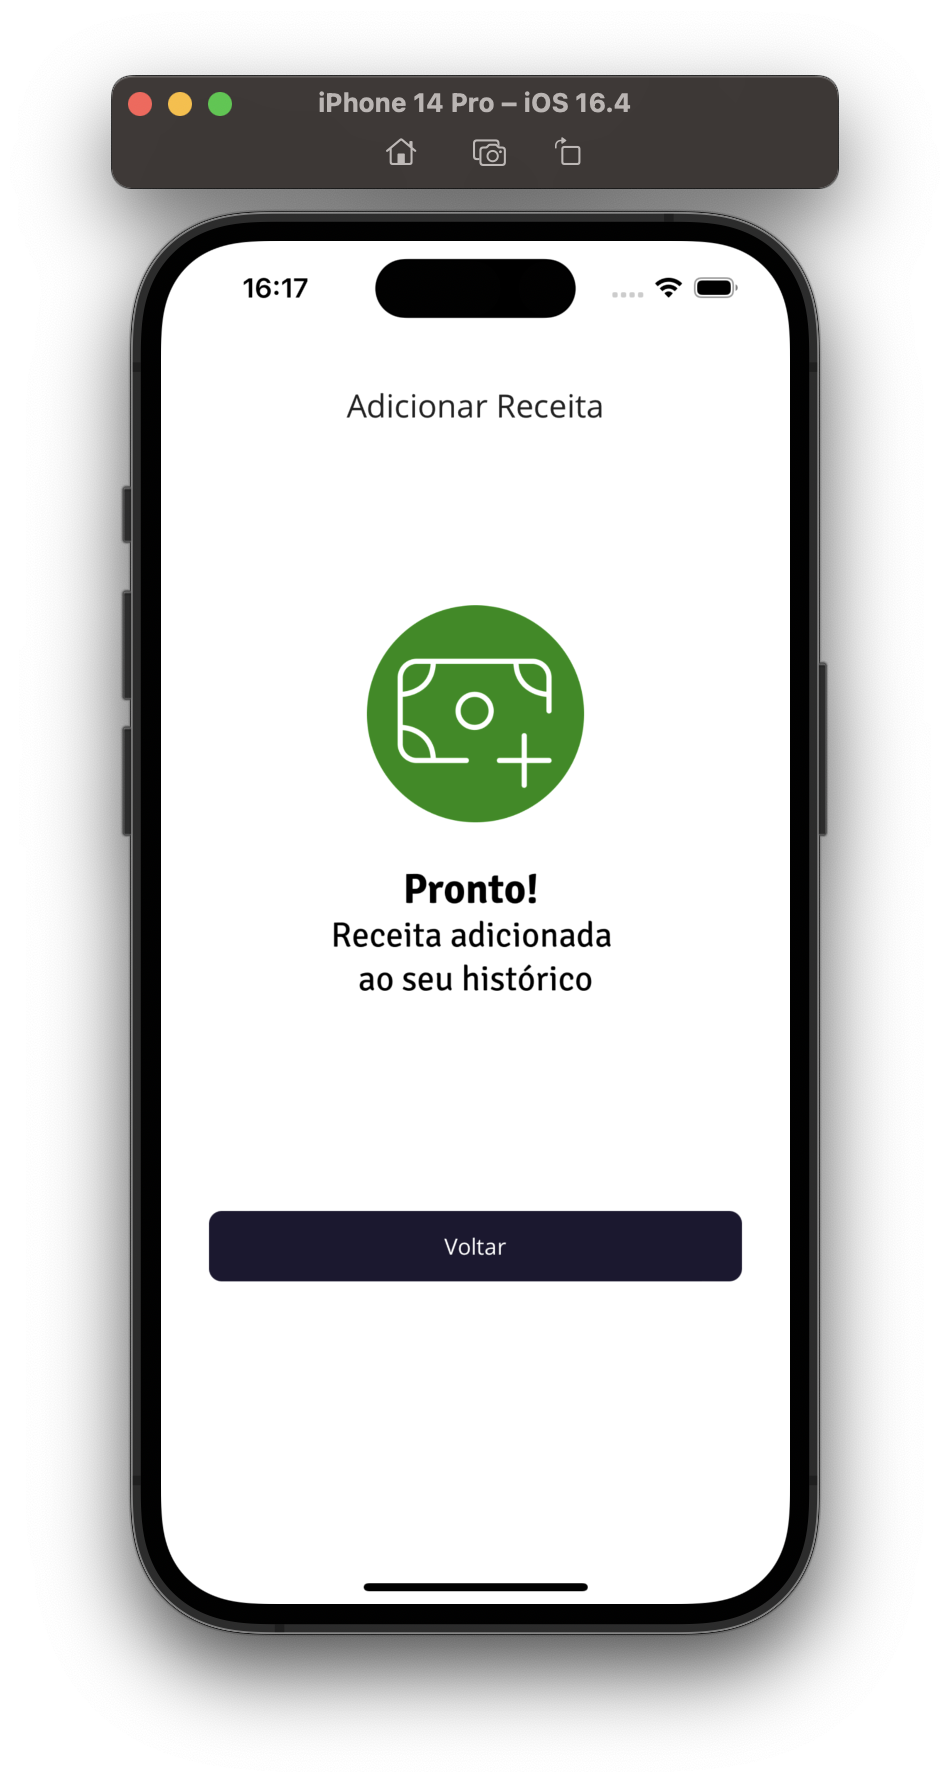
\includegraphics[scale=0.15]{figs/figura27.png}
            \captionof{figure}{Criar Receita II}
            \label{fig:figura27}
        \end{minipage}%
    \end{center}

De acordo com o Menu Principal, ao escolher a opção \textbf{“Adicionar Despesa”} aparecerá a tela da figura 28, contendo dois campos um obrigatório para colocar o valor da despesa, e um campo abaixo que não é obrigatório, para colocar uma descrição sobre a despesa. Ao preencher os campos, basta clicar no botão \textbf{“Adicionar”}. Uma nova tela contendo sucesso na despesa adicionada virá à tona, conforme figura 29.

    \vspace{\baselineskip}
    \begin{center}
        \begin{minipage}{0.4\textwidth}
            \centering
            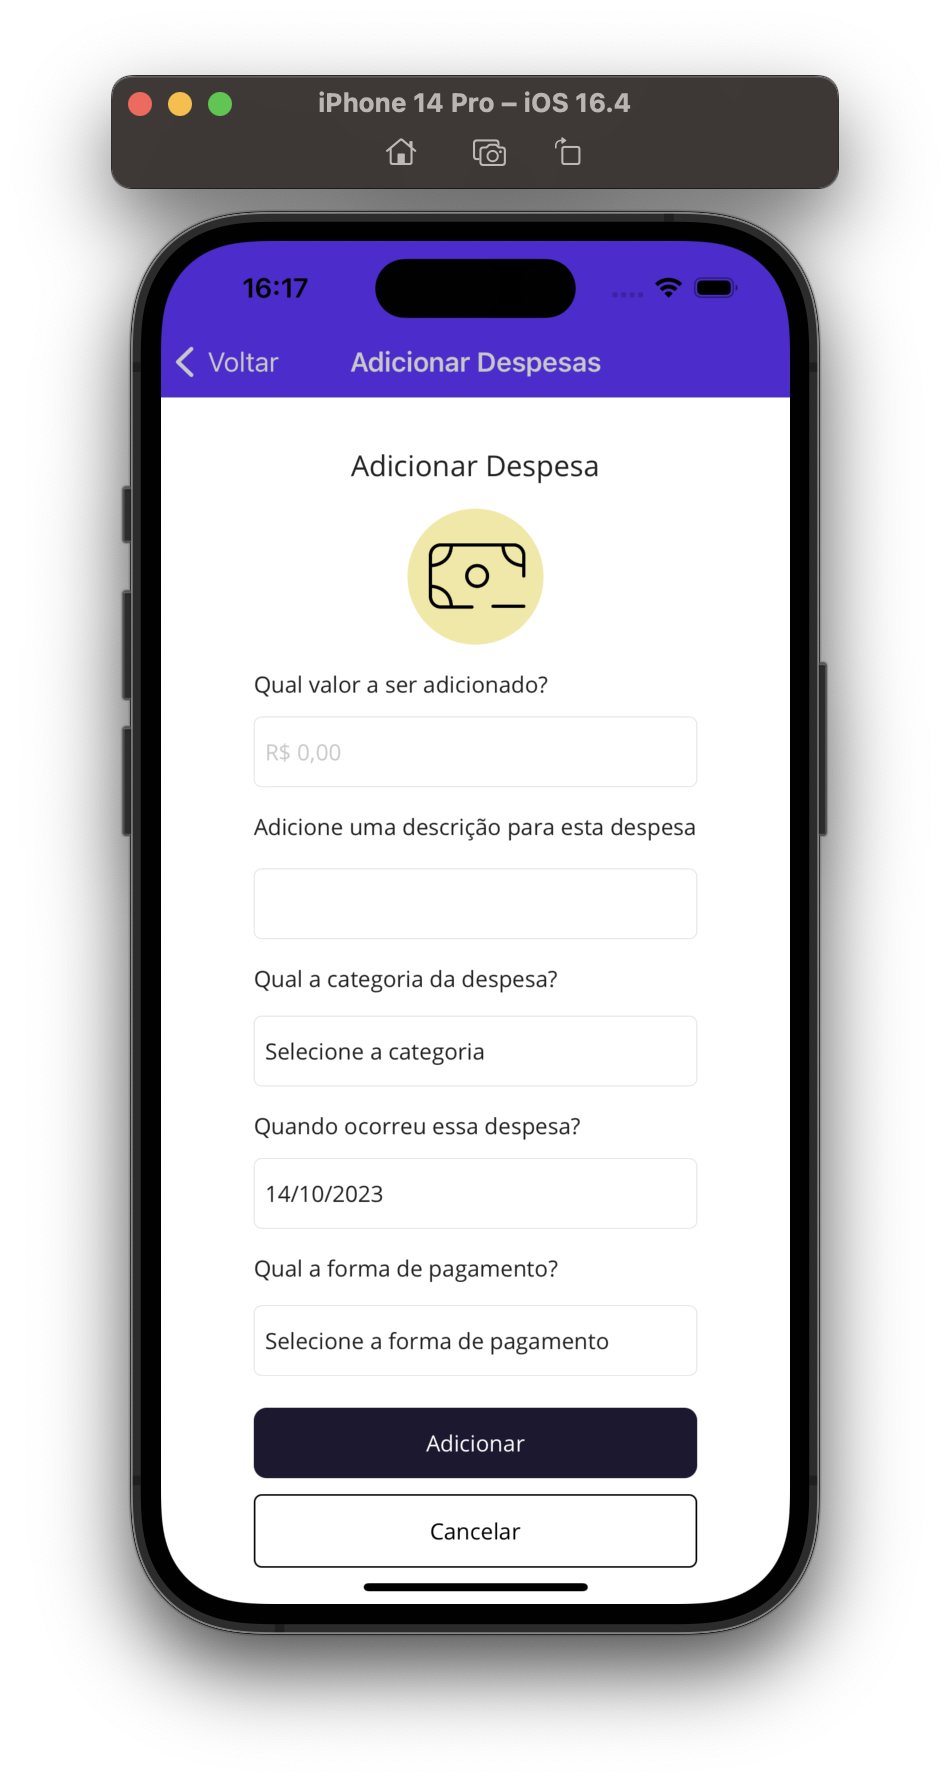
\includegraphics[scale=0.2]{figs/figura28.png}
            \captionof{figure}{Criar Despesa I}
            \label{fig:figura28}
        \end{minipage}%
        \begin{minipage}{0.4\textwidth}
            \centering
            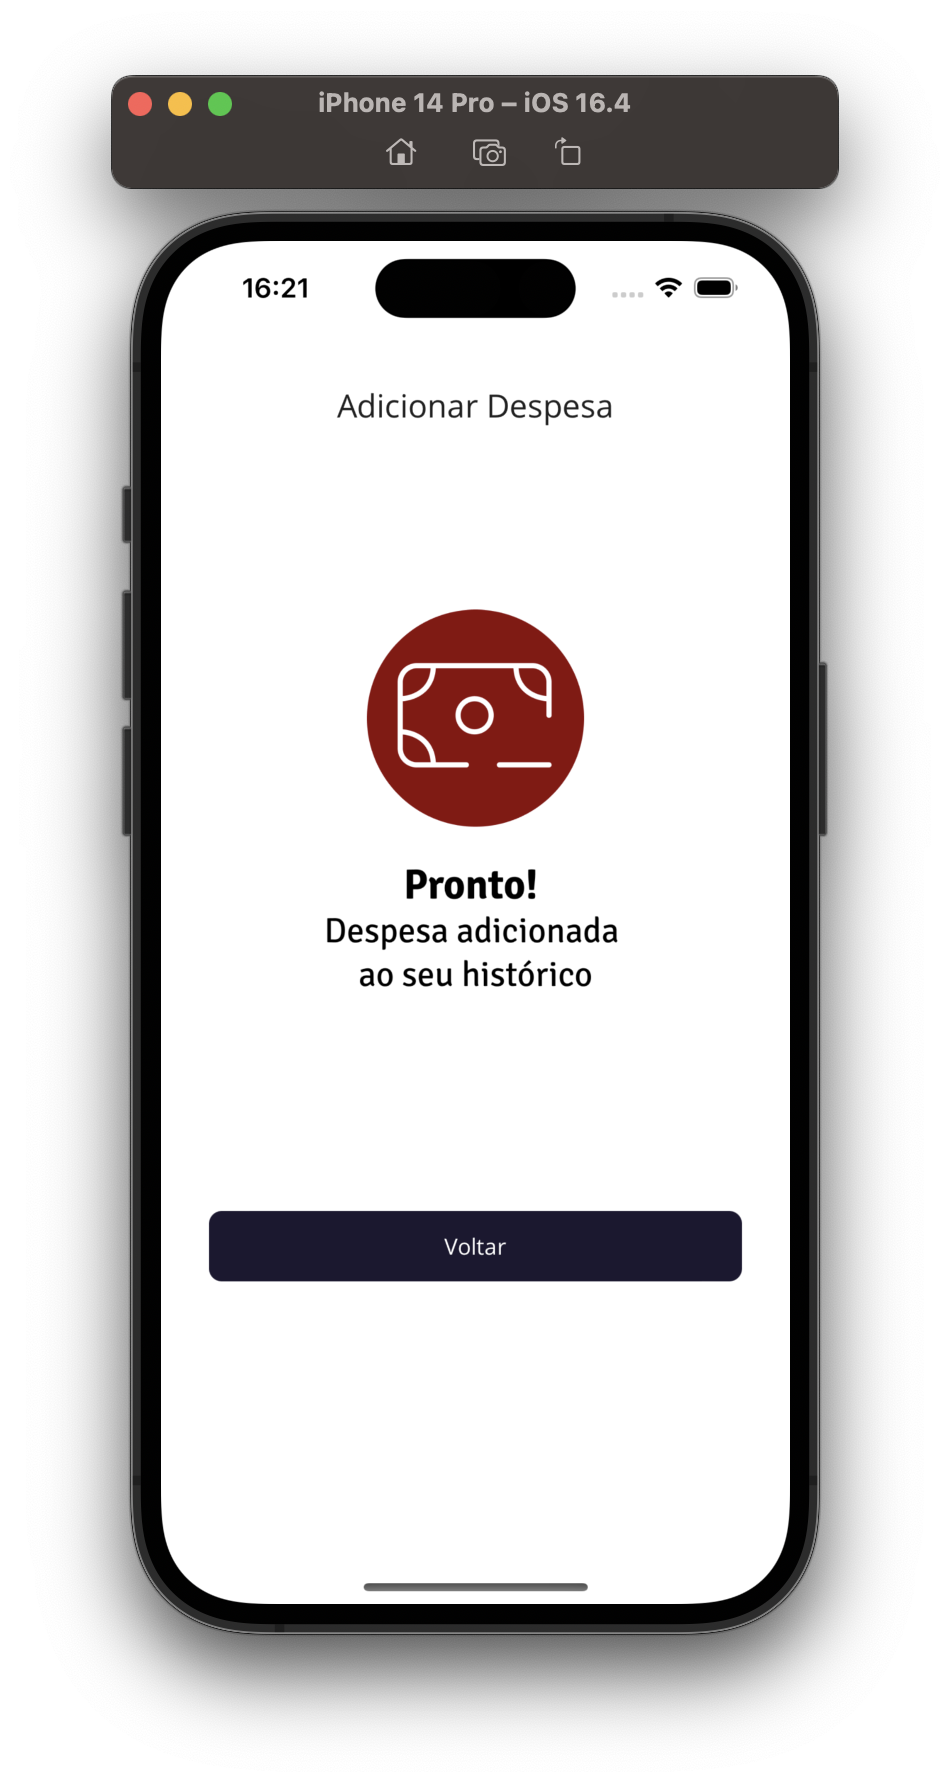
\includegraphics[scale=0.2]{figs/figura29.png}
            \captionof{figure}{Criar Despesa II}
            \label{fig:figura29}
        \end{minipage}%
    \end{center}
    
\subsection{Redefinição de Senha}

Caso o usuário esqueça a senha é possível redefini-la na tela de login clicando no botão \textbf{“Esqueci a Senha”}. Ao fazer isso, aparecerá a primeira tela acima, que contém um campo para inserir o \textit{e-mail} que terá a senha alterada, após inserir o \textit{e-mail} clique no botão \textbf{“Próximo”} abaixo, confome figuras 30 e 31 abaixo. 

    \vspace{\baselineskip}
    \begin{center}
        \begin{minipage}{0.4\textwidth}
            \centering
            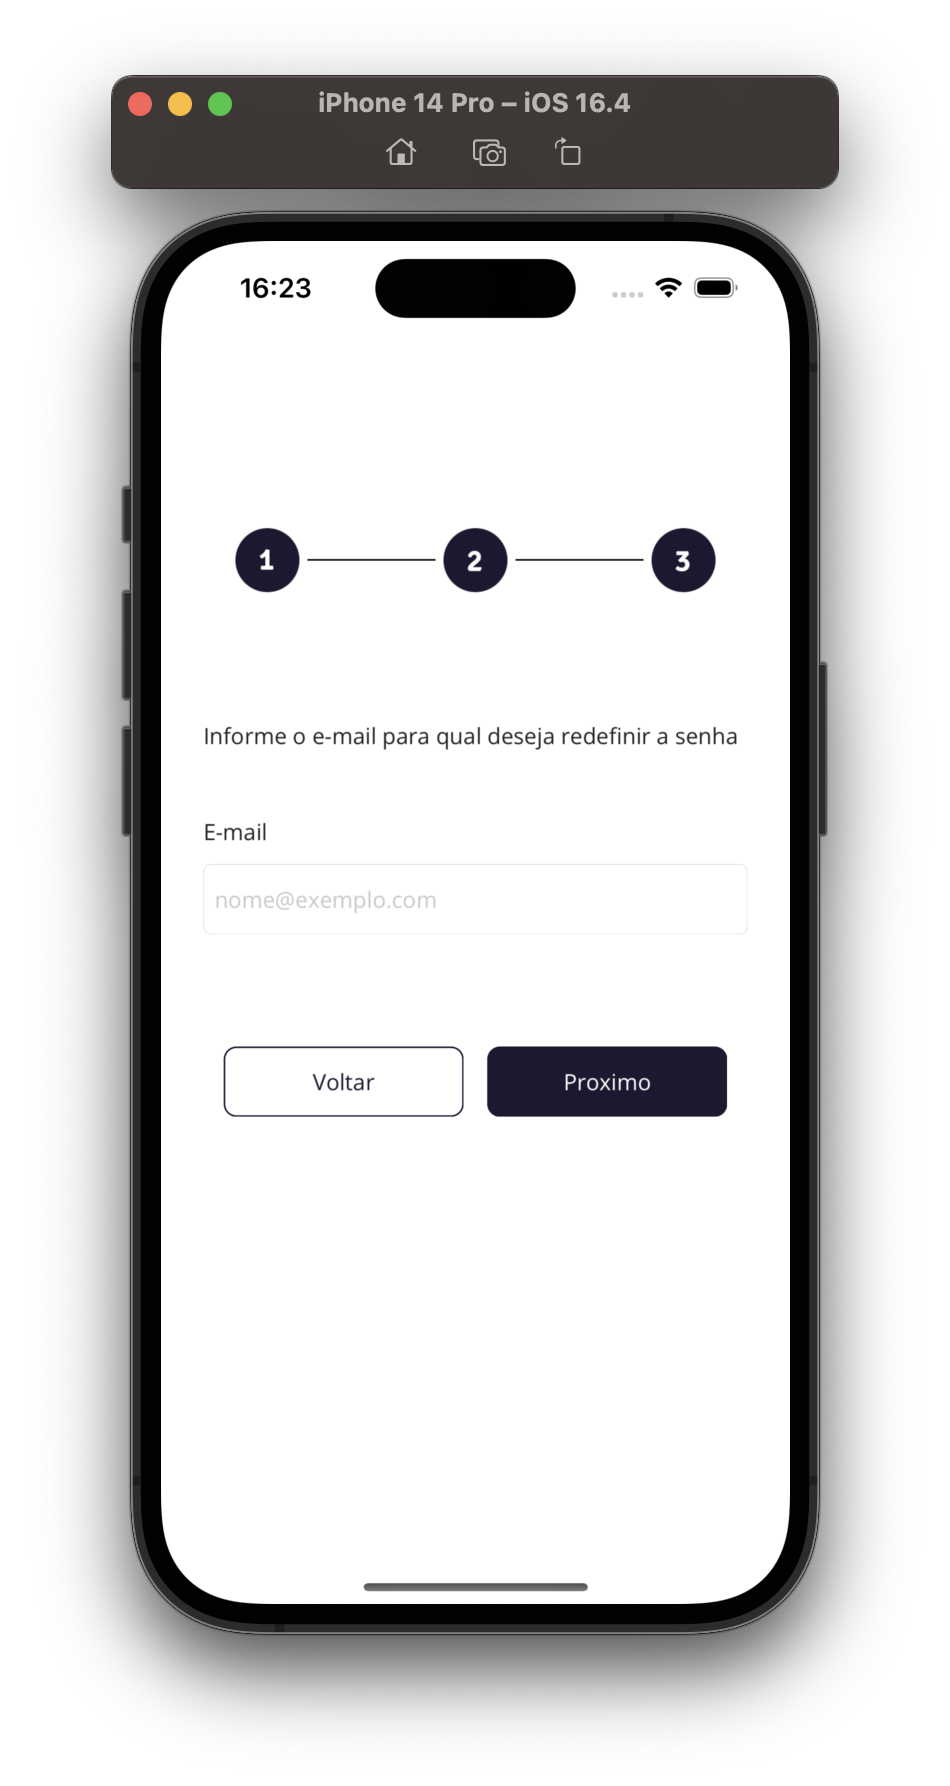
\includegraphics[scale=0.2]{figs/figura30.png}
            \captionof{figure}{Esqueci a Senha I}
            \label{fig:figura30}
        \end{minipage}%
        \begin{minipage}{0.4\textwidth}
            \centering
            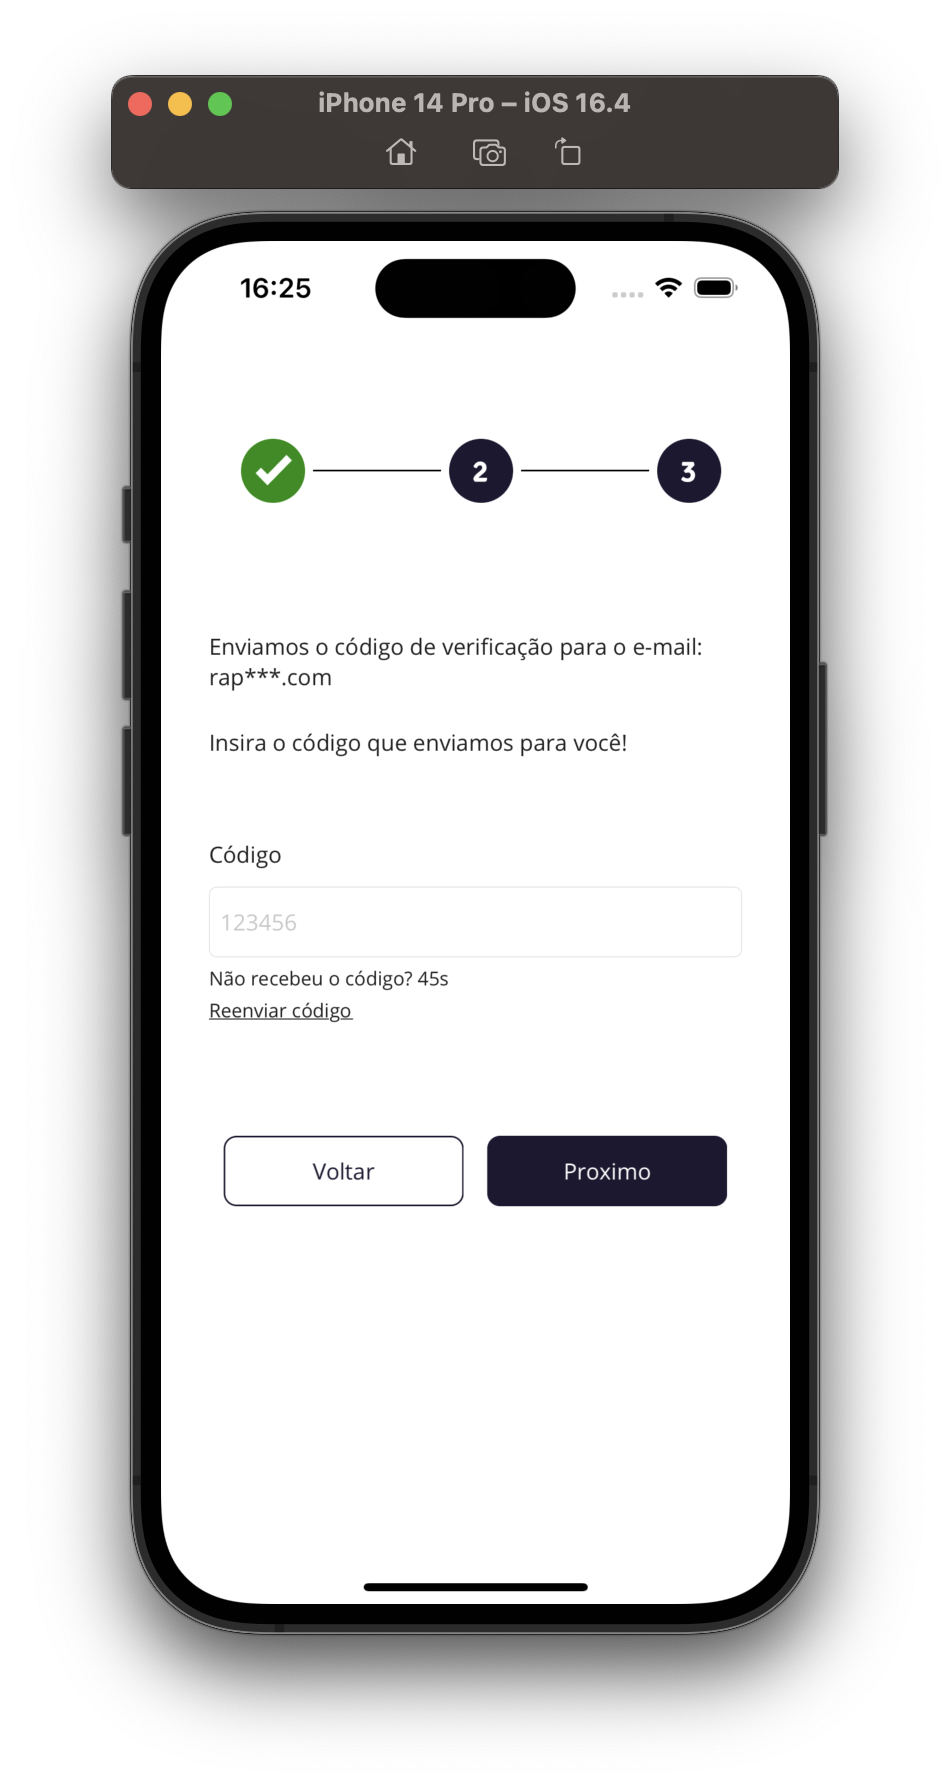
\includegraphics[scale=0.2]{figs/figura31.png}
            \captionof{figure}{Esqueci a Senha II}
            \label{fig:figura31}
        \end{minipage}%
    \end{center}

Consequentemente, uma nova tela aparecerá, contendo um campo para inserir um código que será enviado para o \textit{e-mail} correspondente. Basta inserir esse código no campo e clicar em \textbf{“Verificar”} para confirmar. Caso não tenha recebido o código no \textit{e-mail}, é possível reenviar clicando em \textbf{“Reenviar Código”}, disponível a cada 45 segundos. Na figura 32 e 33, é apresentado a tela de senha redefinida.

    \begin{center}
        \begin{minipage}{0.4\textwidth}
            \centering
            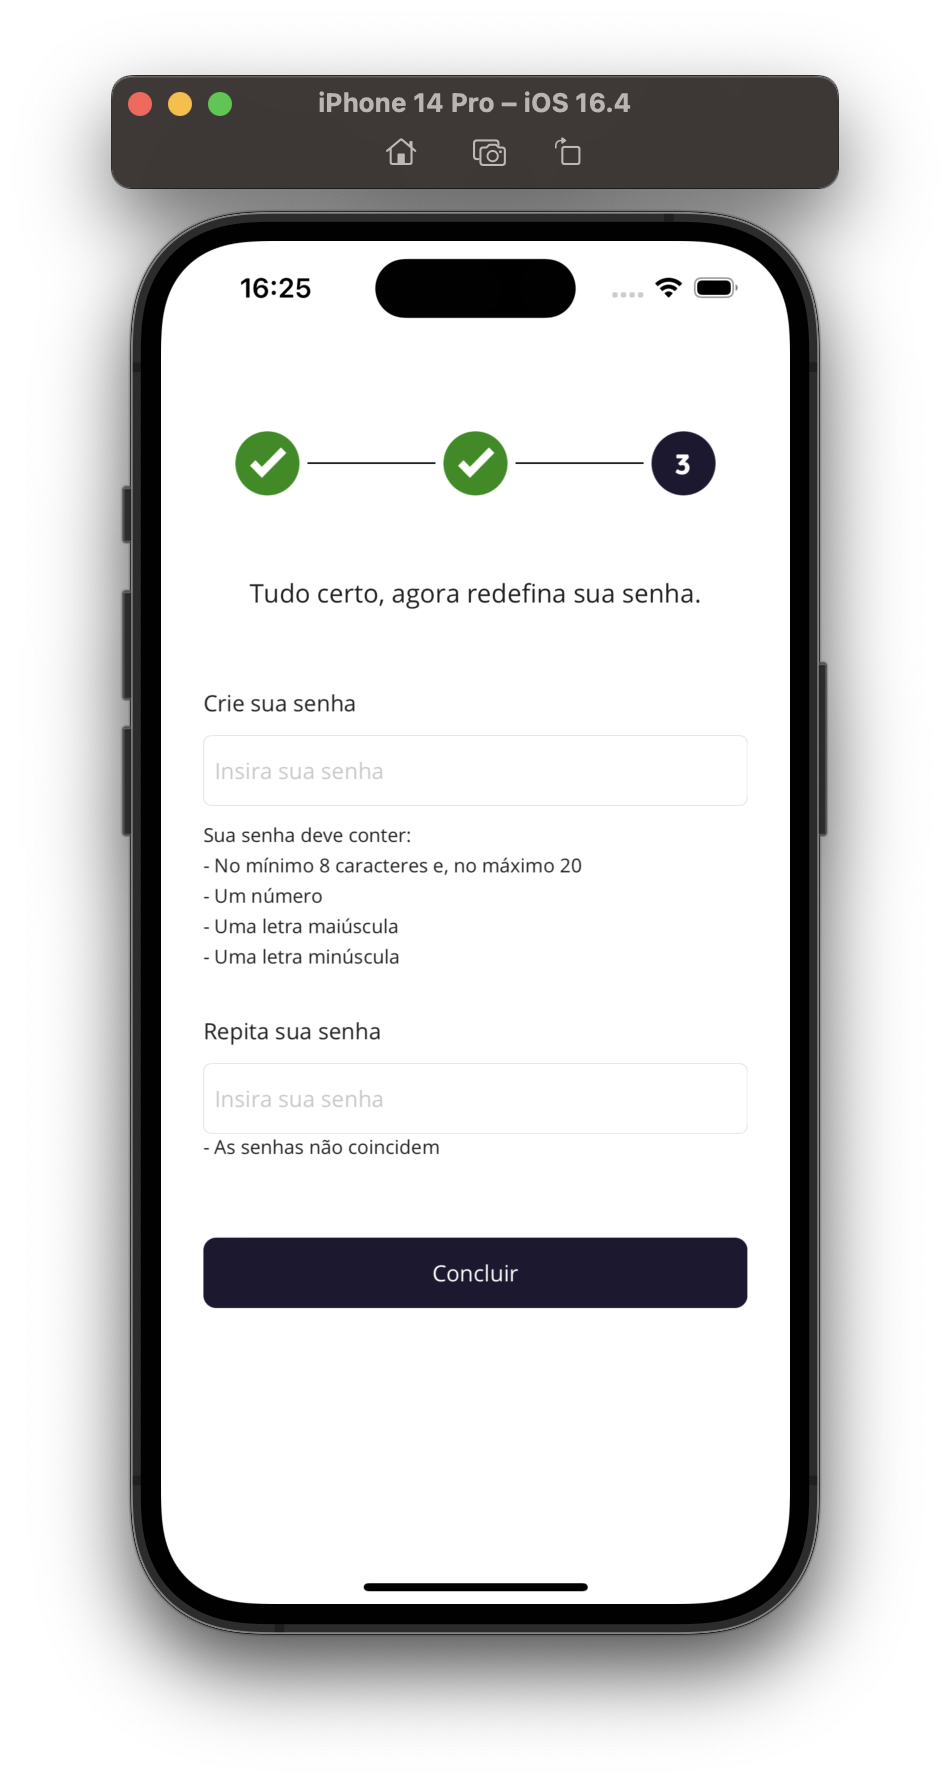
\includegraphics[scale=0.2]{figs/figura32.png}
            \captionof{figure}{Esqueci a Senha III}
            \label{fig:figura32}
        \end{minipage}%
        \begin{minipage}{0.4\textwidth}
            \centering
            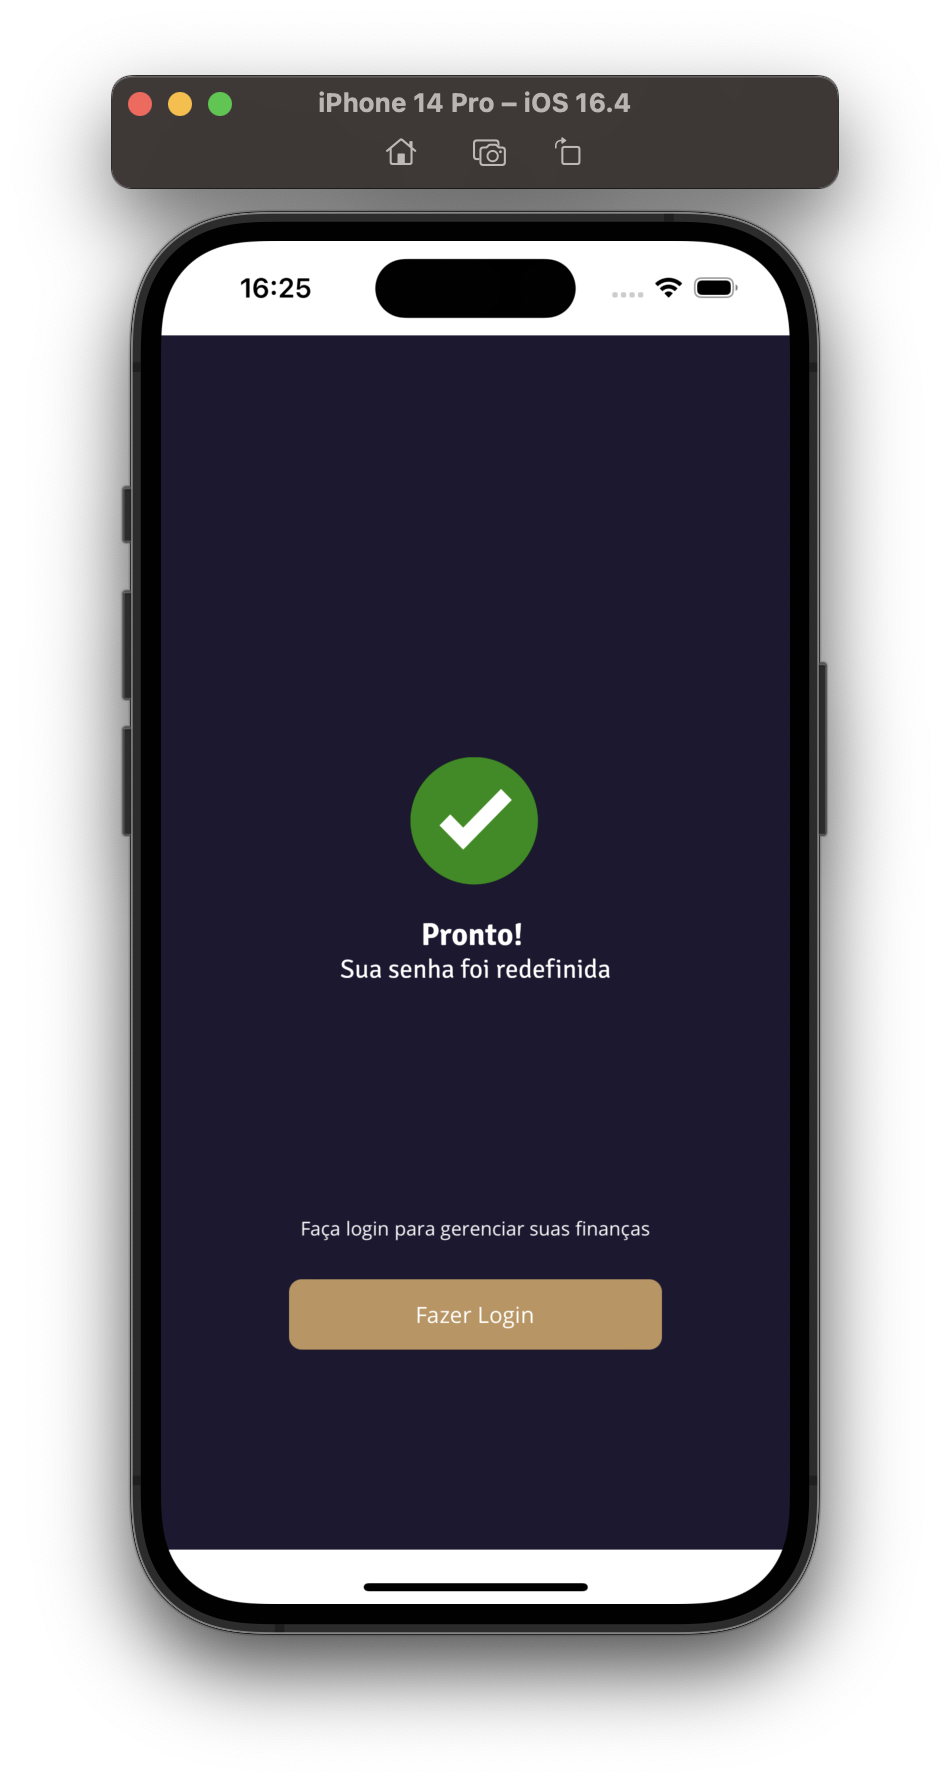
\includegraphics[scale=0.2]{figs/figura33.png}
            \captionof{figure}{Esqueci a Senha IV}
            \label{fig:figura33}
        \end{minipage}%
    \end{center}

Ao clicar um novo código será enviado. Após verificar o código e ter sucesso, uma nova tela surgirá contendo campos para redefinição de senha, o primeiro campo é destinado para inserção da nova senha, que deve respeitar as seguintes exigências: conter no mínimo 8 caracteres, um número, uma letra maiúscula, uma letra minúscula. No campo abaixo repita sua senha caso ambas estejam idênticas clique em \textbf{“Próximo”}. E uma tela apontando sucesso na ação vira à tona, conforme descrito na figura 32. Na figura 34 é apresentada um exemplo da mensagem do código de verificação enviado através do \textit{email}.

    \vspace{\baselineskip}
    \begin{center}
        \begin{minipage}{\textwidth}
            \centering
            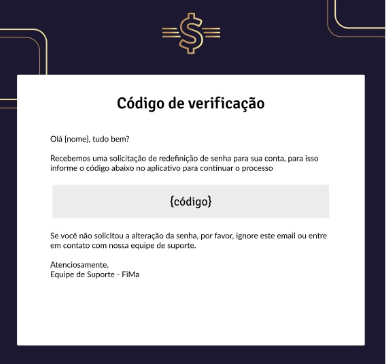
\includegraphics[scale=0.6]{figs/img_6_1.png}
            \captionof{figure}{Esqueci a Senha V}
            \label{fig:figura33}
        \end{minipage}
    \end{center}   

Ao solicitar uma redefinição de senha, a tela acima será exibida, apresentando um campo que requer um código, o qual é gerado através aplicativo. Isso adiciona uma camada adicional às ações. Se não houve solicitação de redefinição de senha, ignore o \textit{e-mail} ou entre em contato com a equipe de suporte.

\subsection{Código Fonte}

Código fonte do projeto: \href{https://github.com/raphaelfrei/financial-manager}{https://github.com/raphaelfrei/financial-manager}

Código fonte do LaTeX: \href{https://github.com/raphaelfrei/fima-final_paper}{https://github.com/raphaelfrei/fima-final\_paper}